%===============================================================================
% LaTeX sjabloon voor de bachelorproef toegepaste informatica aan HOGENT
% Meer info op https://github.com/HoGentTIN/bachproef-latex-sjabloon
%===============================================================================

\documentclass{bachproef-tin}

\usepackage{hogent-thesis-titlepage} % Titelpagina conform aan HOGENT huisstijl
\usepackage{subfigure}
%%---------- Documenteigenschappen ---------------------------------------------
% TODO: Vul dit aan met je eigen info:

% De titel van het rapport/bachelorproef
\title{Secrets management: centraal beheer van gevoelige data}

% Je eigen naam
\author{Rayen Nasra}

% De naam van je promotor (lector van de opleiding)
\promotor{Antonia Pierreux}

% De naam van je co-promotor. Als je promotor ook je opdrachtgever is en je
% dus ook inhoudelijk begeleidt (en enkel dan!), mag je dit leeg laten.
\copromotor{Jan Delamper}

% Indien je bachelorproef in opdracht van/in samenwerking met een bedrijf of
% externe organisatie geschreven is, geef je hier de naam. Zoniet laat je dit
% zoals het is.
\instelling{HoGent}

% Academiejaar
\academiejaar{2020-2021}

% Examenperiode
%  - 1e semester = 1e examenperiode => 1
%  - 2e semester = 2e examenperiode => 2
%  - tweede zit  = 3e examenperiode => 3
\examenperiode{2}

%===============================================================================
% Inhoud document
%===============================================================================

\begin{document}

%---------- Taalselectie -------------------------------------------------------
% Als je je bachelorproef in het Engels schrijft, haal dan onderstaande regel
% uit commentaar. Let op: de tekst op de voorkaft blijft in het Nederlands, en
% dat is ook de bedoeling!

%\selectlanguage{english}

%---------- Titelblad ----------------------------------------------------------
\inserttitlepage

%---------- Samenvatting, voorwoord --------------------------------------------
\usechapterimagefalse
%%=============================================================================
%% Voorwoord
%%=============================================================================

\chapter*{\IfLanguageName{dutch}{Woord vooraf}{Preface}}
\label{ch:voorwoord}

%% TODO:
%% Het voorwoord is het enige deel van de bachelorproef waar je vanuit je
%% eigen standpunt (``ik-vorm'') mag schrijven. Je kan hier bv. motiveren
%% waarom jij het onderwerp wil bespreken.
%% Vergeet ook niet te bedanken wie je geholpen/gesteund/... heeft
%Het volgende onderzoek werd geschreven in het kader van de opleiding Toegepaste Informatica met afstudeerrichting Systeem en Netwerkbeheer. 


%\lipsum[1-2]
Deze thesis ``Secrets management: centraal beheer van gevoelige data`` werd geschreven in samenwerking met het development team van Wolters Kluwer Financial Services. Deze thesis dient als informatieve bron \& als handleiding om de stappen te reproduceren voor te behalen wat met deze proef verwezenlijkt werd. Ik heb dit onderwerp gekozen omdat ik wist dat de resultaten potentieel zouden helpen bij het beheer van gevoelige data doorheen het IT-ecosysteem van Wolters Kluwer.

Deze proef vormt dan ook een hoogtepunt tijdens mijn laatste stappen om mijn studies van de opleiding ``Toegepaste Informatica met afstudeerrichting Systeem en Netwerkbeheer``, te voltooien. Het gekozen onderwerp was zeer interessant om me hierin te verdiepen en kwam met veel uitdagingen die getackeld moesten worden. Dit alles zou ik nooit volbracht hebben zonder de hulp van een aantal personen en hiervoor neem ik graag de tijd om deze mensen te bedanken.

Allereerst wil ik mijn promotor, Antonia Pierreux, bedanken voor alle hulp die ze mij heeft aangeboden door middel van meerdere feedback momenten en mijn teksten meerdere keren door te nemen waarmee ik aanpassingen kon verrichten waar nodig. Ze heeft mij ook sterk gesteund om de juiste beslissingen op tijd te nemen.

Ten tweede wil ik ook graag mijn co-promotor, Jan Delamper \& Herman van der Merwe bedanken voor alle hulp tijdens mijn stage bij Wolters Kluwer \& de mogelijkheid om de proof of concept uit te werken via middelen van het bedrijf.

Als laatste wou ik zeker ook mijn vrienden en medestudenten, Owen van Damme, Emiel van Belle, Olivier Troch en Denys Slyvka  bedanken voor de morele steun die mij heeft blijven motiveren, en de bruikbare feedback die ik heb verwerkt in deze thesis.

%%=============================================================================
%% Samenvatting
%%=============================================================================

% TODO: De "abstract" of samenvatting is een kernachtige (~ 1 blz. voor een
% thesis) synthese van het document.
%
% Deze aspecten moeten zeker aan bod komen:
% - Context: waarom is dit werk belangrijk?
% - Nood: waarom moest dit onderzocht worden?
% - Taak: wat heb je precies gedaan?
% - Object: wat staat in dit document geschreven?
% - Resultaat: wat was het resultaat?
% - Conclusie: wat is/zijn de belangrijkste conclusie(s)?
% - Perspectief: blijven er nog vragen open die in de toekomst nog kunnen
%    onderzocht worden? Wat is een mogelijk vervolg voor jouw onderzoek?
%
% LET OP! Een samenvatting is GEEN voorwoord!

%%---------- Nederlandse samenvatting -----------------------------------------
%
% TODO: Als je je bachelorproef in het Engels schrijft, moet je eerst een
% Nederlandse samenvatting invoegen. Haal daarvoor onderstaande code uit
% commentaar.
% Wie zijn bachelorproef in het Nederlands schrijft, kan dit negeren, de inhoud
% wordt niet in het document ingevoegd.

\IfLanguageName{english}{%
\selectlanguage{dutch}
\chapter*{Samenvatting}
\lipsum[1-4]
\selectlanguage{english}
}{}

%%---------- Samenvatting -----------------------------------------------------
% De samenvatting in de hoofdtaal van het document

\chapter*{\IfLanguageName{dutch}{Samenvatting}{Abstract}} 


Secrets management is een belangrijk onderdeel voor de beveiliging van gegevens. Het impliceert naar applicaties en methodes om gevoelige gegevens te beheren voor gebruik in applicaties, services en andere gevoelige delen van het IT-ecosysteem. Het moet maar één keer gebeuren, dat gegevens met administrator rechten tot een bepaalde server in de verkeerde handen vallen om daarna pijnlijke gevolgen te verdragen. 

Bij Wolters Kluwer wordt TeamCity, een continuous integration \& continuous development (CI/CD) tool, gebruikt voor automatisch applicaties op te bouwen met behulp van een chronologische set van taken die worden opgegeven. Dit onderzoek is vertrokken van een use case met betrekking tot deze tool. Het doel is om gevoelige gegevens beter te beheren in de CI/CD omgeving van TeamCity. Bij het uitvoeren van integratietesten en implementaties, gebruiken build scripts gegevens om toegang te verkrijgen tot externe servers en services. Traditioneel, worden wachtwoorden als veilige parameters op de TeamCity server opgeslagen. Dit biedt vaak niet een hoog genoeg beveiligingsniveau aan. In een productie omgeving van TeamCity met meer dan tienduizend build configuraties waar mogelijk honderden wachtwoorden opgeslagen staan, is het beheer van deze gegevens niet overzichtelijk. Secret management tracht dit probleem op te lossen aan de hand van twee tools die werden opgezet, een on-premise Hashicorp Vault opstelling, en een Microsoft Azure cloud oplossing, Azure Key Vault. Deze tools werden opgezet en geïntegreerd met TeamCity om gegevens te verlenen wanneer deze opgevraagd worden door build scripts. 

Eerst werd een literatuurstudie uitgevoerd om de stand van zaken rond secrets management en cloud oplossingen te verduidelijken. Bij de methodologie werden open-source secret management tools bekeken aan de hand van de MoSCoW-methode. Bij De proof of concept kunt u de stappen volgen hoe beide opstellingen opgesteld zijn voor Wolters Kluwer, een wereldwijde leverancier van professionele informatie, software en diensten. 

Vanuit dit onderzoek werd het duidelijk dat secret management tools gehanteerd kunnen worden om dit en gelijkaardig problemen op te lossen. Gevoelige gegevens die in een TeamCity omgeving staan, kunnen via secret management tools, centraal beheerd worden. Dit vormt een extra abstractielaag tussen de CI/CD tool en gevoelige gegevens. Secret management systemen bieden tegenwoordig veel functionaliteiten aan waarvan er zeker genoeg ruimte is om deze allemaal te onderzoeken in eventueel toekomstige onderzoeken.

%---------- Inhoudstafel -------------------------------------------------------
\pagestyle{empty} % Geen hoofding
\tableofcontents  % Voeg de inhoudstafel toe
\cleardoublepage  % Zorg dat volgende hoofstuk op een oneven pagina begint
\pagestyle{fancy} % Zet hoofding opnieuw aan

%---------- Lijst figuren, afkortingen, ... ------------------------------------

% Indien gewenst kan je hier een lijst van figuren/tabellen opgeven. Geef in
% dat geval je figuren/tabellen altijd een korte beschrijving:
%
%  \caption[korte beschrijving]{uitgebreide beschrijving}
%
% De korte beschrijving wordt gebruikt voor deze lijst, de uitgebreide staat bij
% de figuur of tabel zelf.

\listoffigures
%\listoftables
%\lstlistoflistings

% Als je een lijst van afkortingen of termen wil toevoegen, dan hoort die
% hier thuis. Gebruik bijvoorbeeld de ``glossaries'' package.
% https://www.overleaf.com/learn/latex/Glossaries

%---------- Kern ---------------------------------------------------------------

% De eerste hoofdstukken van een bachelorproef zijn meestal een inleiding op
% het onderwerp, literatuurstudie en verantwoording methodologie.
% Aarzel niet om een meer beschrijvende titel aan deze hoofstukken te geven of
% om bijvoorbeeld de inleiding en/of stand van zaken over meerdere hoofdstukken
% te verspreiden!

%%=============================================================================
%% Inleiding
%%=============================================================================

\chapter{\IfLanguageName{dutch}{Inleiding}{Introduction}}
\label{ch:inleiding}

Bedrijven moeten meer de focus leggen op het beheer van gevoelige data zodat deze ten alle tijden veilig behouden worden. Wanneer applicaties en configuraties in een bedrijf draaien zullen er in bestanden uiteindelijk data komen die er niet zouden mogen zijn. Deze data zou beheerd moeten worden want men weet niet wie bijvoorbeeld binnen een week of twee ditzelfde bestand kan bekijken. Dit soort data noemt men \textit{\textbf{secrets}}. Veel bedrijven falen om dit in te zien en eindigen uiteindelijk met een overvloed aan applicaties en scripts waar gebruikersnamen en wachtwoorden zonder encryptie staan. Deze situatie noemt men een \textit{\textbf{secrets sprawl}}. Deze twee termen komen in onderdeel~\ref{sec:secrets management} aan bod en worden daar verder uitgelegd.

Doorheen de jaren zijn er een aantal applicaties verschenen die dit probleem proberen op te lossen door alle secrets in een centrale locatie op te slaan. Vanuit deze centrale node kan men authenticatie verlenen wanneer secrets nodig zijn. 

Een belangrijke workflow binnen software bedrijven is \textit{continuous integration \& continuous development (CI/CD)}. Hierbij worden continu applicaties opgebouwd die aangestuurd worden door een chronologische set van taken. Deze taken bevatten soms dan gevoelige gegevens die over het hoofd worden gezien. Elke gebruiker die toegang heeft om deze taken te beheren kan deze gegevens zien.

%De inleiding moet de lezer net genoeg informatie verschaffen om het onderwerp te begrijpen en in te zien waarom de onderzoeksvraag de moeite waard is om te onderzoeken. In de inleiding ga je literatuurverwijzingen beperken, zodat de tekst vlot leesbaar blijft. Je kan de inleiding verder onderverdelen in secties als dit de tekst verduidelijkt. Zaken die aan bod kunnen komen in de inleiding~\autocite{Pollefliet2011}:

\section{\IfLanguageName{dutch}{Probleemstelling}{Problem Statement}}
\label{sec:probleemstelling}

Bij Wolters Kluwer wordt TeamCity, een CI/CD tool gebruikt voor automatisch applicaties op te bouwen met behulp van een chronologische set van taken die worden opgegeven. Deze taken bevatten soms secrets die niet in encryptie staan. Dit is geen best practice en zou voorkomen moeten worden. TeamCity biedt de mogelijkheid aan om gevoelige data te maskeren in de vorm van \textit{password parameters} maar alsnog is dit geen optimale manier van werken. Bij Wolters Kluwer zijn er momenteel 12966 build configuraties aanwezig waar zeker secrets in allerlei plaatsen zijn opgeslagen. Dit vormt de probleemstelling dat geen deftig overzicht is van waar secrets staan. Mogelijks staan er ook secrets zonder encryptie in parameter velden / build scripts. Het beheren van secrets is een beveiligingsmaatregel die vaak over het hoofd wordt gezien. Er bestaan applicaties die als doel hebben om deze gevoelige data af te schermen bij de werking van automatisering, CI/CD applicaties en container omgevingen. Deze applicaties bieden een oplossing aan voor gecentraliseerd beheer van secrets. Omdat Wolters Kluwer een hybride aanpak neemt met cloud en on-premise, zal er voor beide omgevingen een tool worden gebruikt. Deze dienen als fundament om het nut van deze technologie waar te nemen, en om deze verder te integreren binnen het bedrijf.




%Uit je probleemstelling moet duidelijk zijn dat je onderzoek een meerwaarde heeft voor een concrete doelgroep. De doelgroep moet goed gedefinieerd en afgelijnd zijn. Doelgroepen als ``bedrijven,'' ``KMO's,'' systeembeheerders, enz.~zijn nog te vaag. Als je een lijstje kan maken van de personen/organisaties die een meerwaarde zullen vinden in deze bachelorproef (dit is eigenlijk je steekproefkader), dan is dat een indicatie dat de doelgroep goed gedefinieerd is. Dit kan een enkel bedrijf zijn of zelfs één persoon (je co-promotor/opdrachtgever).

\section{\IfLanguageName{dutch}{Onderzoeksvraag}{Research question}}
\label{sec:onderzoeksvraag}

%Wees zo concreet mogelijk bij het formuleren van je onderzoeksvraag. Een onderzoeksvraag is trouwens iets waar nog niemand op dit moment een antwoord heeft (voor zover je kan nagaan). Het opzoeken van bestaande informatie (bv. ``welke tools bestaan er voor deze toepassing?'') is dus geen onderzoeksvraag. Je kan de onderzoeksvraag verder specifiëren in deelvragen. Bv.~als je onderzoek gaat over performantiemetingen, dan 

Bij deze bachelorproef horen enkele onderzoeksvragen waar een antwoord op wordt gezocht, deze zijn als volgt:

\begin{itemize}
    \item Welke open-source applicatie kan er gebruikt worden om \textbf{secrets} te beheren?
    \item Welke cloud oplossing kan er gebruikt worden om \textbf{secrets} te beheren?
    \item Welke opstelling on-premise of via cloud oplossing, geeft een betere werking voor de use case met TeamCity?
%    \item Kunnen deze opstellingen geautomatiseerd worden via reproduceerbare tactieken?
\end{itemize}


\section{\IfLanguageName{dutch}{Onderzoeksdoelstelling}{Research objective}}
\label{sec:onderzoeksdoelstelling}

%Wat is het beoogde resultaat van je bachelorproef? Wat zijn de criteria voor succes? Beschrijf die zo concreet mogelijk. Gaat het bv. om een proof-of-concept, een prototype, //een verslag met aanbevelingen//, een vergelijkende studie, enz.

Dit onderzoek heeft tot doel het belang aan te tonen van secrets management binnen IT. Voor een Proof of Concept worden twee kandidaten gekozen om uitgewerkt te worden waar één als cloud oplossing, en één on-premise. Deze proof of concept zou ook een begin moeten zijn om het secrets probleem aan te pakken dat zich voordoet bij Wolters Kluwer met de CI/CD tool TeamCity. Het vormt ook als handleiding om de genomen stappen te reproduceren. Deze beide opstellingen trachten het probleem op te lossen met de gegeven reëel use case, en dienen aan als startpunt om na deze thesis verder geïntegreerd te worden binnen het bedrijf.

%Als laatste is het doel ook dat het bedrijf waar de concrete opstellingen uitgevoerd worden, verder kunnen met de integratie van deze \textit{Proof of Concept} om deze in een productie omgeving te brengen zodat deze ten volle macht gebruikt kan worden.

\section{\IfLanguageName{dutch}{Opzet van deze bachelorproef}{Structure of this bachelor thesis}}
\label{sec:opzet-bachelorproef}

% Het is gebruikelijk aan het einde van de inleiding een overzicht te
% geven van de opbouw van de rest van de tekst. Deze sectie bevat al een aanzet
% die je kan aanvullen/aanpassen in functie van je eigen tekst.

De rest van deze bachelorproef is als volgt opgebouwd:

In Hoofdstuk~\ref{ch:stand-van-zaken} wordt een overzicht gegeven van de stand van zaken binnen secrets managements \& cloud computing, op basis van een literatuurstudie.

In Hoofdstuk~\ref{ch:methodologie} wordt de methodologie toegelicht om met de MoSCoW-methode, een kandidaat te selecteren voor de on-premise opstelling.

In Hoofdstuk~\ref{ch:poc} wordt een proof of concept opgezet met de gekozen tools. Deze tools worden geconfigureerd \& geïntegreerd met TeamCity waar de concrete probleemstelling ligt.

% TODO: Vul hier aan voor je eigen hoofstukken, één of twee zinnen per hoofdstuk

In Hoofdstuk~\ref{ch:conclusie}, tenslotte, wordt de conclusie gegeven en een antwoord geformuleerd op de onderzoeksvragen. Daarbij wordt ook een aanzet gegeven voor toekomstig onderzoek binnen dit domein.
\chapter{\IfLanguageName{dutch}{Stand van zaken}{State of the art}}
\label{ch:stand-van-zaken}

% Tip: Begin elk hoofdstuk met een paragraaf inleiding die beschrijft hoe
% dit hoofdstuk past binnen het geheel van de bachelorproef. Geef in het
% bijzonder aan wat de link is met het vorige en volgende hoofdstuk.

% Pas na deze inleidende paragraaf komt de eerste sectiehoofding.

%Dit hoofdstuk bevat je literatuurstudie. De inhoud gaat verder op de inleiding, maar zal het onderwerp van de bachelorproef *diepgaand* uitspitten. De bedoeling is dat de lezer na lezing van dit hoofdstuk helemaal op de hoogte is van de huidige stand van zaken (state-of-the-art) in het onderzoeksdomein. Iemand die niet vertrouwd is met het onderwerp, weet nu voldoende om de rest van het verhaal te kunnen volgen, zonder dat die er nog andere informatie moet over opzoeken \autocite{Pollefliet2011}.
\section{Secrets Management}
\label{sec:secrets management}
Om te verstaan wat \textbf{secrets management} inhoudt, worden de termen \textbf{secrets} en \textbf{secrets sprawl} weer verduidelijkt. Secrets impliceert een verzameling van gevoelige gegevens. Deze dienen als sleutel om digitale authenticatie uit te voeren, om toegang te krijgen tot een systeem \autocite{Dadgar2018}. Enkele voorbeelden zijn:

\begin{itemize}
    \item Gebruikersnaam en wachtwoord
    \item API tokens
    \item SSH keys
    \item Database inloggegevens
\end{itemize}

Deze gegevens zullen een secret sprawl veroorzaken wanneer deze niet onderhouden worden op de juiste manier. Secret sprawls ontstaan wanneer sensitieve gegevens, in allerlei plaatsen gebruikt worden om mee te werken. Bijvoorbeeld in automatisatie processen (Ansible, Puppet, Chef), containerized applications (Kubernetes, Red Hat OpenShift, Docker), Continuous Integration/Continuous Deployment (CI/CD) (TeamCity, Jenkins). Vroeg of laat belanden bestanden met onbewerkte tekst van gevoelige data in versiebeheer systemen, applicatie systemen of worden deze als lokale variabele gebruikt. Veel problemen ontstaan wanneer een bedrijf veel te laat beseft dat ze met een secret sprawl zitten, maar één van de grootste problemen is dat het bedrijf in meerdere locaties gevoelige gegevens heeft staan en dat er geen duidelijk overzicht is van waar deze gegevens zitten. Het bedrijf zal dan ook niet weten welke personen toegang hebben om deze gegevens te bekijken \autocite{Tozzi2020} \autocite{Dadgar2018}. 
\newline 


Secrets management streeft naar een situatie waar secret sprawls vermeden worden, de gegevens geëncrypteerd zijn, dat de distributie van deze gegevens beheerd worden vanuit een gecentraliseerde locatie en als laatste dat deze gegevens gebruikt kunnen worden bij automatische processen zonder enige manuele tussenkomst. \textcite{Somerfield2015} legde uit hoe de uitdagingen die deze problemen stelden, werden aangegaan. Hier wordt het \textit{Orchestrator Decryption} model uitgelegd \autocite{Somerfield2015}. 

\subsection{Orchestrator Decryption} 

\begin{figure}[htbp]
\centerline{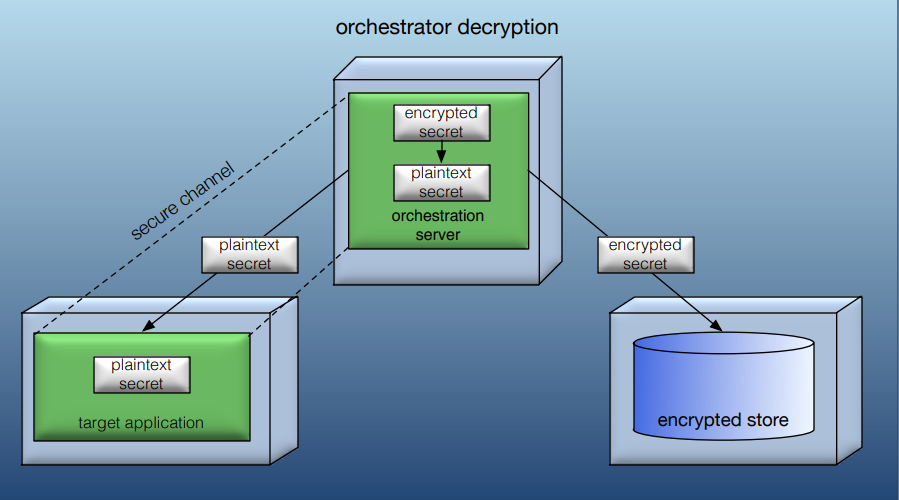
\includegraphics[width=400]{bachproef/img/orchestrator decryption.png}}
\caption{Orchestrator Decryption \autocite{Somerfield2015}}
\label{fig}
\end{figure}

Bij \textbf{orchestrator decryption} kijken we vooral naar \textit{configuration management tools} zoals ansible, chef, puppet. Deze applicaties kunnen met een tussenkomst van bijkomende applicaties gevoelige data veilig houden wanneer deze niet gebruikt worden, deze zijn in rust geëncrypteerd. Wanneer de geëncrypteerde secret wordt opgeroepen bij een opdracht wordt deze door de orchestration tool naar een \textit{plaint text} secret gedecrypteerd, met andere woorden wordt deze omgevormd tot onbewerkte tekst. Een voorbeeld van een orchestration georiënteerde tool is ansible. Deze tool kan gebruik maken van ansible vault om een vorm van secret management aan te gaan maar wordt gelimiteerd door een aantal factoren waardoor het binnen het model van \textit{Orchestrator decryption} blijft \autocite{Somerfield2015}. Om dit duidelijk uit te leggen, wordt in het algemeen uitgelegd wat ansible is en waarvoor deze tool gebruikt wordt. Verder wordt er ook uitgelegd hoe ansible vault hierop inspeelt. \newpage

\subsection{Ansible}  
\label{ch:ansible}

Ansible\footnote{\href{https://www.ansible.com}{Ansible website}} is een open-source, configuration management tool (CMT) die door Red Hat\footnote{\href{https://www.redhat.com}{Red Hat website}} onderhouden wordt sinds 2015. Ansible is tegenwoordig op de voorgrond als het om geautomatiseerd configuratie, coördinatie en beheer van computer systemen gaat. Tegenwoordig is ansible de meest gebruikte CMT waar het applicaties zoals Chef, Salt en Puppet overtreft \autocite{Rayome2019}. Het is ook handig voor simpele gebruikers die alledaagse taken willen uitvoeren binnen simpele netwerken, en niet alleen op één computer. Deze tool geeft je de mogelijkheid om binnen een complex netwerk van computers, vanuit één centraal punt, configuraties te deployen en systemen te beheren. Dit lost problemen op zoals bijvoorbeeld, wanneer men op verschillende computers het zelfde doel wilt bereiken zonder deze taak manueel opnieuw en opnieuw te doen op elke computer. Men kan via een centrale computer opdrachten versturen naar één of meerdere locaties tegelijkertijd. Hierdoor wordt ook het concept van menselijke fout vermeden.

In Ansible wordt er een onderscheid gemaakt tussen de control node en de managed node. De control node is een computer die ansible draait waar alle taken uit verzend worden. Deze taken voeren wijzigingen uit op de managed nodes. Ansible's manier van werken is allereerst een verbinding vast te leggen met de managed nodes, daarna wordt tijdelijk een programma gepushed dat uitgevoerd wordt tijdens deze verbinding. Deze programma’s noemen ansible modules. Bij het einde van een taak wordt de module lokaal op de node verwijderd en sluit ansible de verbinding met de node. Ansible is \textit{agentless} gebaseerd. Dit wilt zeggen dat op de managed nodes geen ansible applicatie aanwezig moet zijn die de configuraties verkrijgt en verwerkt. Ansible maakt gebruik van \textit{connection plugins} waaruit \textbf{SSH} (Secure Shell) de meest gebruikte is. Deze worden gebruikt om een verbinding vast te leggen met linux / unix hosts. Voor Windows hosts wordt \textbf{WinRM} (Windows Remote Management) gebruikt \autocite{RedHatAnsible2021}. 

\begin{figure}[htbp]
\centerline{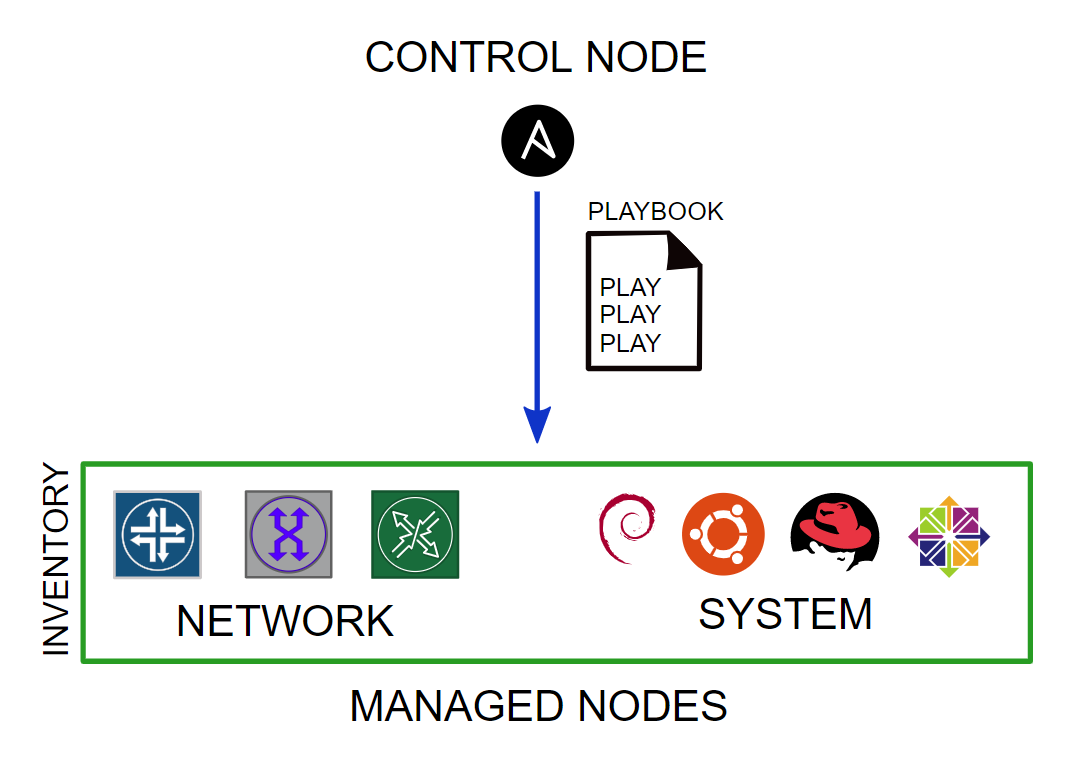
\includegraphics[width=250]{bachproef/img/AnsibleArchitecture.png}}
\caption{Werking ansible met control en managed nodes \autocite{Coding2019}}
\label{fig}
\end{figure}
\newpage
Omdat Ansible een tool omtrent automatisatie is, heeft deze tool dan ook instructies nodig. De instructies die ansible uitvoert zijn idempotent. Dit wilt zeggen wanneer bij een instructie een opdracht wordt uitgevoerd, maar er valt niets te wijzigingen in het systeem, zal ansible hier niets doen. Ansible zal deze stap overslaan en de volgende opdracht proberen uitvoeren \autocite{Coding2019}. Deze instructies worden als taken opgenomen in een \textbf{YAML} (Yet another Markup Language) bestand \autocite{ingerson80yet}. Een jaar na de introductie van het YAML formaat is de betekenis van het acroniem verandert naar (YAML Ain't Markup Language) \autocite{VugtYAML}, dat is inderdaad een recursief acroniem. %Hieronder wordt er een voorbeeld gegeven van een inventory file en een playbook. De \textit{inventory file} kan een generiek bestand zijn zonder extensie, een ansible playbook is altijd in een YAML bestandsformaat. 


\begin{figure}[hbtp]
    \caption{Voorbeeld inventory file ansible}
    %\label{code.1}
    \begin{lstlisting}[language=yaml,frame=single]
        [web]
        be-dev-ansible-01
        be-dev-ansible-02
        
        [web:vars]
        ansible_python_interpreter=/usr/bin/python3
        ansible_ssh_user=John 
        ansible_ssh_pass=JohnSecure123
    \end{lstlisting}
    \label{fig:inventorypass}
\end{figure}
De inventaris afgebeeld op figuur \ref{fig:inventorypass}, impliceert dat de machines, \textit{be-dev-ansible-01} en \textit{be-dev-ansible-02}, met de extra variabelen opgeroepen kunnen worden als groep web. Hierdoor gebruiken playbooks volgende python versie, volgende SSH gebruikersnaam en het bijbehorende wachtwoord bij het uitvoeren van volgende taken.


\begin{figure}[hbtp]
    \caption{Voorbeeld ansible playbook}
    %\label{code.1}
    \begin{lstlisting}[language=yaml,frame=single]
    1.	---
    2.	- hosts: web
    3.	  tasks:
    4.      - name: permit traffic on port 10000-10001/tcp
    5.          firewalld:
    6.          port: 10000-10001/tcp
    7.          permanent: yes
    8.          state: enabled
    9.	    - name: ensure nginx is at the latest version
    10.	      apt: name=nginx state=latest
    11.	    - name: start nginx
    12.	      service:
    13.	          name: nginx
    14.	          state: started
    \end{lstlisting}
    \label{fig:playbookvb}
\end{figure}

In figuur \ref{fig:playbookvb} wordt er geïllustreerd hoe ansible voor de groep web, volgende taken gaat uitvoeren. Allereerst wordt er gezien of de TCP poorten 10000 en 10001 open staan, indien dit het geval is gebeurt er hier niets en gaat het playbook verder. Dit wordt aangeduid door het \textit{state: enabled} gedeelte. Verder wordt er gekeken om nginx te installeren via de \textit{command-line utility commando} apt, als nginx reeds geïnstalleerd is zal er gekeken worden of die van de laatste versie is. Na het uitvoeren of het overslaan van deze taak wordt er voor gezorgd dat nginx gestart is als dit niet het geval is. Moest er bijvoorbeeld iets intern mis gaan bij een van de taken, zal deze in het output scherm als een \textit{fatal error} verschijnen met een boodschap waarom dit gebeurt is en voor welke host.

In het vorige voorbeeld werd er aangetoond hoe problematisch het is wanneer \textbf{secrets} in een productieomgeving in allerlei bestanden als onbewerkte tekst terechtkomen. Wanneer er meerdere playbooks worden aangemaakt die elk gevoelige data bevatten om de automatisatie te behouden. Is het onvermijdelijk dat deze vroeg of laat op source control terechtkomen. Eens dat gebeurt, is het al te laat. Via audit kan men vorige versies bekijken van \textit{commits} en gevoelige data in de vorm van onbewerkte tekst zien \autocite{Wehner2015}. Iedereen die in deze \textit{public} of \textit{private repository} zit kan de secrets zo bekijken, en men weet niet wie deze gegevens reeds bekeken heeft. 

\subsection{Ansible Vault} 

In het geval van ansible en playbooks biedt ansible vault een mogelijke oplossing, Ansible Vault\footnote{\href{https://docs.ansible.com/ansible/2.9/user\_guide/vault.html}{Ansible Vault website}} is een tool voor ansible dat bestanden met gevoelige data encrypteert. Dit biedt de mogelijkheid aan zodat alle taken kunnen uitgevoerd worden tijdens ansible taken die gegevens gebruiken die niet zichtbaar mogen zijn. Ansible zal de bestanden automatisch decrypteren tijdens looptijd, mits de sleutel voorzien is. Via één of meerdere wachtwoorden kan men inhoud encrypteren en decrypteren \autocite{RedhatAnsibleVault}. Dit lost het probleem op dat gegevens niet meer zichtbaar zijn voor de buitenwereld. Maar ansible vault lost jammer genoeg het probleem niet volledig op. Wanneer ansible modules verstuurt worden naar een managed node, worden deze tijdelijk opgeslagen in een verborgen directory. Hier staan deze gegevens zonder encryptie. Dit wilt zeggen dat de gebruikte data, bijvoorbeeld wachtwoorden, overgezet worden op het bestandssysteem van de remote host. Zoals eerder verteld kan ansible alternatieve connection plugins gebruiken om een verbinding met een remote host vast te leggen. Als men SSH gebruikt zal de data geëncrypteerd en veilig zijn tijdens het versturen van de modules. Dit beveiligt de data tegen potentiële \textbf{sniffing attacks}. Dit is een tactiek die gebruikt wordt om data te achterhalen tijdens netwerk connectiviteit. Zo kunnen gegevens in onbewerkte tekst achterhaald worden \autocite{Passi2018}. Eens data verzonden is, kan het zijn dat deze toch op de remote host geschreven worden zonder enige encryptie. Dit kan bijvoorbeeld gebeuren wanneer de omgevingsvariabele \textbf{ansible\_keep\_remote\_files} gebruikt wordt. Hiermee blijven gebruikte modules op de remote host staan. Moest deze omgevingsvariabele niet gebruikt worden kan het nog altijd zijn wanneer een verlies van connectiviteit zich plaatsvindt, de modules op de remote host niet verwijderd zijn. Deze blijven daar tot ze manueel verwijderd worden \autocite{GB2018}. Verder is er ook nog de mogelijkheid om de omgevingsvariabele \textbf{no\_log} te gebruiken en deze op \textit{true} te stellen. Dit zorgt er voor dat wanneer de modules weergeven worden in het systeem log, de gevoelige data verborgen blijft. Dit wordt afgebeeld op figuur \ref{fig:nolog} \autocite{GB2018}.
\newpage

Zoals bij ansible vault getoond werd, is het een last om er voor te zorgen dat secrets niet gelekt worden bij het uitvoeren van taken en bij het beheren van bestanden met deze data. Het kanaal waarmee secrets verstuurd worden is niet altijd veilig genoeg om op te vertrouwen. Het beheer van alle secrets via de ansible vault manier is dan ook niet efficiënt in een ondernemingsomgeving. Er is geen vorm van rotatie zodat gegevens na zoveel tijd aangepast worden. Als een persoon een wachtwoord vergeet voor een bestand geëncrypteerd door ansible vault zijn die gegevens zo goed als verloren. De nadelen zijn hier veel te groot en het grootste probleem bij secrets management van secrets centraal te beheren is hier niet opgelost. 

\begin{figure}[htbp]
\centerline{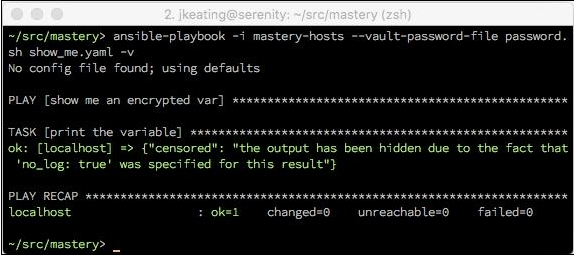
\includegraphics[width=300]{bachproef/img/nolog.png}}
\caption{gebruik van 'no\_log: true' in ansible \autocite{GB2018}}
\label{fig:nolog}
\end{figure}

\newpage
\subsection{Application-Pull}

\begin{figure}[htbp]
\centerline{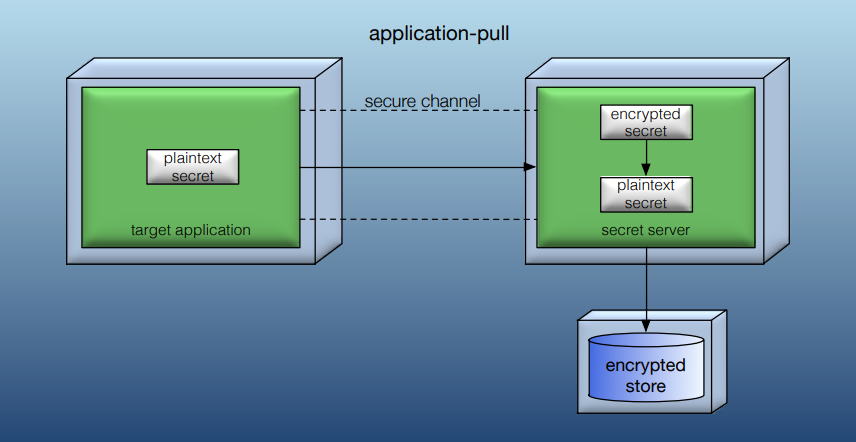
\includegraphics[width=400]{bachproef/img/application-pull.png}}
\caption{Application-pull \autocite{Somerfield2015}}
\label{fig}
\end{figure}

Een model dat meer aansluit bij het principe van secrets management is \textbf{application-pull}. Hierbij kan een persoon, of een service, zich via een systeem laten authenticeren om toegang te krijgen tot een locatie waar secrets beheerd worden. Via een beleid wordt er bepaald of toegang verleend wordt. Alles gebeurt nu ook vanuit een gecentraliseerd punt. Dit is een verbetering en een stevig concept dat meer aansluit bij secret management. Deze applicaties garanderen een aantal sterke punten, namelijk:

\begin{itemize}
    \item \textit{Central management}
    \item \textit{Access policies}
    \item \textit{Auditing}
    \item \textit{Ephemeral credentials}
    \item \textit{Compartmentalization}
    \item \textit{Facilitates rotation}
\end{itemize}

Dit zijn belangrijke kenmerken voor een secrets management systeem. Vault van Hashicorp is één van de applicaties die \textit{application-pull} duidelijk verwoordt. Volgens \textcite{Somerfield2015} was dit in 2015 een applicatie die al in de juiste richting ging \autocite{Somerfield2015}. We zijn ondertussen, bij het schrijven van deze thesis, zes jaar verder.  
%Hier zijn een aantal \textbf{secret management platform} die vandaag de dag het dichtst zijn om \textbf{secrets} de baas te zijn waar ook over besproken zal worden \autocite{Morris2020}:
\newpage

\subsection{Hashicorp Vault}
\label{sec:Hashicorp vault}

Hashicorp, Inc.\footnote{\href{www.hashicorp.com}{Hashicorp website}} is een softwarebedrijf opgericht door Mitchell Hashimoto en Armon Dadgar in 2012. Ze bieden open-source tools en commerciële producten aan die ontwikkelaars de mogelijkheid aanbiedt om applicaties op te zetten in een multi-cloud omgeving. Hashicorp staat bekend voor Vagrant en Terraform. Maar nu gaat de focus naar Vault. Vault is een \textbf{secret management tool} die ontworpen is om gecentraliseerd gevoelige gegevens te bewaren en toegang te beheren tot deze data in een omgeving met weinig vertrouwen. Het kan gebruikt worden om gevoelige data op te slaan en om dynamisch toegang te genereren voor andere applicaties en services \autocite{Lugger2020}. Hashicorp is al jaren mee om een oplossing te zoeken tot de probleemstelling die gemaakt werd door \textbf{secrets} te beheren via een optimale manier. Via vault hopen zij het grootste deel van deze problemen aan te gaan via drie niveau 's \autocite{Dadgar2018}.

\subsubsection{Niveau 1: Central Management}
In het eerste niveau wilt vault het \textbf{secrets sprawl} probleem tegengaan, hiermee worden alle \textbf{secrets} in een centraal punt verzameld. Deze gegevens worden gedecrypteerd en zo behouden gedurende de drie stadia van data, namelijk: \textit{at rest}, \textit{in transit}, en \textit{in use}. Gegevens belanden niet meer in source control of dergelijke zaken, en staan veilig en gedecrypteerd in één locatie. Een volgend punt is de toegangscontrole die vergemakkelijkt wordt. In tegenstelling tot een bitbucket repository van een bedrijf waar iedereen toegang tot heeft, kan men beheren welke gegevens gezien en gebruikt kunnen worden door welke applicaties, alsook welke personen. Daarnaast is er ook een \textit{audit trail} die gebruikt kan worden om na te gaan welke gegevens gebruikt zijn geweest door applicaties en personen \autocite{Dadgar2018}.

\subsubsection{Niveau 2: Dynamic Secret}

Bij dit volgende niveau wordt de probleemstelling benaderd waarbij niet alle applicaties juist omgaan met secrets. Men kan optimaal het eerste niveau beheren maar toch secrets laten lekken door applicaties die deze gegevens gaan gebruiken. Applicaties kunnen bijvoorbeeld secrets loggen naar een log systeem, ze kunnen in diagnostische rapporten verschijnen of zelf opgenomen worden door monitor applicaties als deze actief zijn. Hieruit kan een besluit genomen worden dat applicaties een slechte werking kunnen hebben met secrets. Om dit probleem op te lossen maakt vault gebruik van \textit{ephemeral credentials}. Dit zijn vluchtige gegevens die dynamisch aangemaakt kunnen worden. Met andere woorden zullen deze gegevens na een bepaalde duur niet meer geldig zijn. Een volgende stap is dat men deze gegevens gaat compartimentaliseren om duidelijker de bron van schade terug te vinden. Als voorbeeld heeft men 40 web servers die allemaal dezelfde gegevens gebruiken om een connectiviteit vast te leggen met een databank, een \textbf{shared secret}. Eens deze gegevens gelekt worden kan men moeilijk weten van waar deze gegevens gelekt zijn geweest. Als men voor elke web server unieke gegevens gebruikt, zal men weten dat er bijvoorbeeld een lek heeft plaatsgevonden bij webserver zeven. Hiermee kan men dan ook de gegevens die webserver zeven gebruikt intrekken en deze isoleren van de andere webservers. Indien alle webservers dezelfde gegevens zouden gebruikt hebben, zouden al deze webservers onderbroken worden. Met andere woorden \textit{dynamic secrets} gaan boven \textit{shared secrets} \autocite{Dadgar2018}.

\subsubsection{Niveau 3: Encrypt as a Service}

Het laatste niveau dat wordt aangekaart is hoe externe applicaties die gebruik maken van vault, data verkrijgen, en deze data juist gebruiken wanneer deze \textit{at rest} zijn. Men kan bijvoorbeeld kijken naar de situatie wanneer encryptie sleutels beheerd worden in vault. Deze sleutels worden aan applicaties verleend om cryptografie toe te passen op de data. Applicaties implementeren cryptografie vaak niet op een juiste manier, dit is ook iets dat \textcite{duong2011cryptography}
%Thai Duong en Juliano Rizzo 
hebben aangekaart in een onderzoek waar ze aantonen hoe cryptografie misbruikt wordt in de security designs van een groot deel van het web. Hun focus ging naar ASP.NET. Vault heeft dit probleem waargenomen en stelde zich de vraag hoe ze het voorkomen om een verzameling van encryptie sleutels te beheren en deze te verlenen aan applicaties waar zij cryptografie uitvoeren. Dit is een concept dat is uitgegroeid tot een hele service genaamd \textit{Encrypt as a Service}. Hier geeft vault de mogelijkheid om \textit{named keys} aan te maken. Dit kunnen bank gegevens zijn, krediet kaart gegevens, een identificatienummer, ... Hier worden \textit{High level API's} gebruikt om transactie 's uit te voeren met deze gegevens zoals encrypteer, verifieer, teken. Bij applicaties waar zulke transacties gebeuren, wordt vault via een API aangeroepen om deze zorgvuldig uit te voeren, zonder de nood van de \textit{named keys} en hun gegevens te delen met de applicatie. De implementatie voor dit proces wordt behandeld door vault, men moet applicaties niet vertrouwen om \textit{high level operations} zorgvuldig uit te voeren, en de key management gebeurt ook nog altijd door vault. Deze worden afgeschermd bij de andere applicaties \autocite{Dadgar2018}. 

Via vault werd er aangetoond hoe secrets management een vooruitgang heeft gehad voor secrets te beheren. Door de opkomst van cloud computing zijn er ook een tal secrets management systemen ontstaan in de vorm van cloud oplossingen. Azure Key Vault is een voorbeeld, van Microsoft Azure. Maar eerst wordt in het algemeen uitgelegd wat cloud computing is en de basis hier omtrent.
\newpage


\section{Cloud Computing}
\label{sec:cloud oplossingen}

Volgens de \textbf{\textit{national institute of standards and technology}}\footnote{\href{https://www.nist.gov/}{Nist website}} is cloud-computing (CC) een model, waar services aangeboden worden via een netwerk toegang (internetverbinding) naar een gedeelde netwerkpool van configureerbare ICT-middelen. Deze zijn makkelijk en snel lanceerbaar met het minimum aan moeite zonder enige tussenkomst met de service provider \autocite{mell2011nist}. Dit impliceert dat applicaties, services en data door een eindgebruiker gebruikt kunnen worden via een gebruikersinterface \autocite{malathi2011cloud}. Een heel simpel voorbeeld is het gebruik van e-mail services, zoals: Outlook, Gmail, ... Bij deze zaken heb je juist een computer met een internet verbinding nodig. Dan kan je gebruik maken van de e-mail services die worden aangeboden door een externe provider. Verder duidt het \textit{national institute of standards and technology} aan dat het CC model opgebouwd is uit vijf essentiele karakteristieken, namelijk:

\begin{itemize}
    \item On-demand self service
    \item Broad network access
    \item Measured service
    \item Resource pooling
    \item Rapid elasticity
\end{itemize}

Bij \textbf{\textit{on-demand self service}} zullen de gebruikers met de gegeven resources automatisch kunnen werken zonder tussenkomst van de service provider. Verder zorgt \textbf{\textit{broad network access}} ervoor dat de aangeboden services toegankelijk zijn via een netwerkverbinding. \textbf{\textit{Measured Service}} volgt het principe dat de gebruiker betaalt voor wat men gebruikt, zo is er geen verspilling van resources. Dit wordt ook wel eens het \textbf{\textit{pay as you go}} model genoemd. \textbf{\textit{Resource Pooling}} volgt het principe dat service providers computing resources aan meerdere consumenten aanbieden met de noden van de klant voor het gebruik van virtuele en fysieke middelen. Het geeft een meerwaarde dat gebruikers de zelfde apparatuur gebruiken voor zowel gebruiker als provider. Als laatste is \textbf{\textit{Rapid elasticity}} de eigenschap dat een service \textit{elastisch} moet zijn wat impliceert dat een service moet kunnen op- en afschalen om aan de gegeven capaciteit te voldoen. Met andere woorden is het belangrijk dat er bij piekbelasting moet kunnen worden opgeschaald zonder enige moeite om voor geen storingen te zorgen, verder bij rustige perioden moet er dan ook weer kunnen worden afgeschaald. In kort zijn dit de vijf hoofd kenmerken van cloud computing. Het model is ook nog opgebouwd uit drie \textbf{service models} en vier \textbf{deployment models} die later in deze thesis aan bod komen \autocite{mell2011nist}.
\newpage

Tegenwoordig kent de wereld een aantal grote spelers bij het aanbieden van cloud oplossingen waaronder:

\begin{itemize}
    \item Amazon Web Services (AWS) \footnote{\href{https://aws.amazon.com/}{Amazon AWS website}}
    \item Microsoft Azure \footnote{\href{https://azure.microsoft.com/nl-nl/}{Microsoft Azure website}}
    \item Google Cloud \footnote{\href{https://cloud.google.com/}{Google Cloud website}}
    \item Alibaba Cloud \footnote{\href{https://eu.alibabacloud.com/en}{Alibaba Cloud website}}
    \item Digital Ocean \footnote{\href{https://www.digitalocean.com/}{Digital Ocean website}}
\end{itemize}

 Dit zijn voorbeelden van cloud providers die een public cloud omgeving aanbieden. Hier betaalt de gebruiker voor het gebruik van de ter beschikking gestelde resources. Cloud providers zoals AWS en Microsoft Azure hanteren het eerder besproken concept van \textbf{\textit{Measured Service}} zelfs. Ze bieden hun services aan volgens een \textbf{\textit{Pay as you go}} subscriptie model zodat men betaalt voor wat men uiteindelijk gebruikt. Zo worden bijvoorbeeld bedrijven niet aangerekend voor resources die ze niet gebruiken op het moment zelf. maar ze hebben wel de toegang om deze te gebruiken. Dit is handig wanneer bijvoorbeeld doorheen de dag veel gebruik gemaakt wordt van bepaalde resources maar tijdens de nacht de curve daalt. Verder proberen cloud providers de \textbf{\textit{Quality of Service}} optimaal te houden tegenover de eindgebruiker in een dynamische omgeving. Door de voortdurende groei en optimalisatie van cloud computing komen telkens nieuwe mogelijkheden aan bod voor ontwikkeling van applicaties en systemen \autocite{mell2011nist}. CC zorgt er uiteindelijk voor dat bedrijven kunnen opereren zonder een ouderwetse infrastructuur. Natuurlijk zijn er mogelijkheden waarmee er gecombineerd kan worden met reeds bestaande infrastructuur. Hierdoor noemt het ook cloud \textbf{oplossingen}, voor elk probleem en elke situatie is er wel een oplossing.
\newpage

\subsection{Deployment Models}
\label{sec:Deployment models}

\subsubsection{Public cloud}

\begin{figure}[htbp]
\centerline{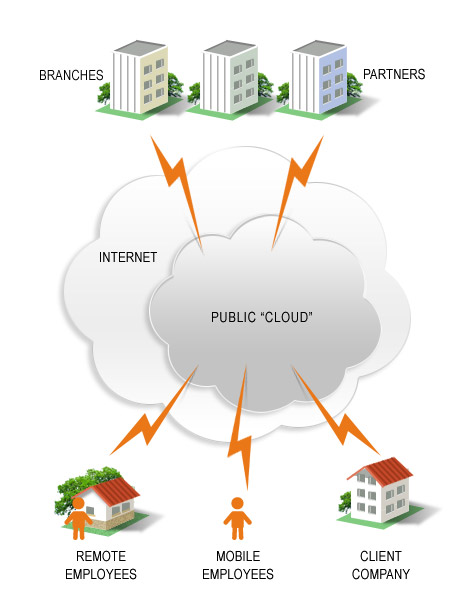
\includegraphics[width=250]{publicCloud.jpg}}
\caption{\textit{public cloud figuur \autocite{mizitechinfo}}}
\label{fig}
\end{figure}

Eerder werd er gesproken over een aantal cloud providers. Deze bieden namelijk diensten aan, die als eerder vermeld een \textbf{\textit{Pay as you go}} gebaseerde subscriptie volgen. Gebruikers betalen bijvoorbeeld voor de \textbf{CPU cycles}, of met andere woorden het gebruik van processor krachten, gebruikte opslag of de gebruikte bandbreedte. Het grootste voordeel hiervan is dat bedrijven zich geen zorgen moeten maken om uitbreidingskosten of het beheren van deze infrastructuur. Er moet niet worden gekeken om een locatie te voorzien, om deze machines te laten draaien want dit wordt al gedaan voor de eindgebruiker. Indien er toch wordt uitgebreid voor meer rekenkrachten of als dit juist verminderd wordt, is dit maar binnen enkele muisklikken te doen \autocite{Sullivan2015PAYG}. Takken zoals beveiliging wordt door de cloud provider optimaal verzorgd. Dit is natuurlijk ook een risico dat gebruikers en bedrijven op zich nemen omdat hun gegevens door een externe partij beheerd wordt. Voor veel bedrijven is dit een serieuze afknapper samen met het feit dat de resources gedeeld worden met andere gebruikers \autocite{cbtnuggets_2019}. Wanneer een bepaalde cloud provider het slachtoffer wordt van een gegevens lek, is de kans natuurlijk groot dat de gegevens van de gebruikers gelekt worden. Dit is geen prettige scenario wanneer gevoelige data geëncrypteerd zou moeten zijn. Door gebruik te maken van een public cloud is dit iets wat bedrijven niet altijd onder controle hebben voor wanneer dit evenement plaats vindt. Door het gebruik van andere \textbf{deployment models} kan dit wel nog tegengewerkt worden.


\subsubsection{Private Cloud}

In tegenstelling tot public cloud waar bedrijven hun data niet volledig in eigen beheer hebben, is dit bij private cloud wel het geval. Hierbij worden cloud computing services aangeboden ofwel via het internet of via een intern privé netwerk uitsluitend aan bepaalde gebruikers. Dit staat niet open voor andere consumenten. Zoals bij de public cloud worden dezelfde services en mogelijkheden aangeboden. In deze instantie met de extra controle die beschikbaar gesteld worden, die via een computerinfrastructuur, die on-premise wordt gehost, gebruikt kan worden. Voor de beveiliging kan het niveau van diepgang zelf gekozen worden door de bedrijven dankzij zowel interne firewalls als interne hosting. Zo zijn de acties en gegevens afgeschermd tegenover externe providers. Private clouds worden vooral gebruikt door grote bedrijven om makkelijk toegang te bieden tot de gegevens over het hele netwerk van het bedrijf. Er zijn twee service modellen die geleverd kunnen worden binnen private cloud. Als eerste kan \textbf{\textit{Infrastructure as a Service (IaaS)}} gebruikt worden waar infrastructurele resources ter beschikking gesteld worden. Verder kan \textbf{\textit{Platform as a Service (PaaS)}} ook gehanteerd worden waar allerlei toepassingen door het bedrijf geleverd kunnen worden via het netwerk. In een verder stuk worden deze twee service modellen verder uitgelegd \autocite{MicrosoftAzurePrivateCloud} \autocite{cbtnuggets_2019} \autocite{goyal2014public}.

Natuurlijk ontstaan er ook enkele voordelen en nadelen bij het hanteren van een private cloud. Zo zijn de kosten bij het opzetten van een private cloud hoger dan bij het gebruik van een public cloud door het kopen van de infrastructuur en de locatie voorzieningen hiervan. De software en de tewerkstelling van personeel voor de taken om deze te beheren en te onderhouden. Een van de belangrijkste voordelen is dan wel de veiligheid van de privacy van data, er zijn geen externe partijen betrokken bij het opereren van de data binnen het bedrijf.

\subsubsection{Community Cloud}

Community cloud is een vorm waar niet te veel in wordt verdiept. Het volgt een \textbf{deployment model} waar het principe geldt dat een cloud computing oplossing wordt toegewezen aan een kleine \textit{community} met dezelfde business doeleinden, door een andere \textit{community}, of een externe partij, of een combinatie van beide gevallen \autocite{jimenez2013supporting}. Dit kan bijvoorbeeld een gezamenlijk project zijn waar \textit{bedrijf a} een ander bedrijf, \textit{bedrijf b}, een bepaalde service voor zich laat uitwerken zodat \textit{bedrijf a} op andere zaken kan focussen. Zoals een webshop waar het gedeelte voor af te rekenen onderhouden wordt door een ander bedrijf.


\subsubsection{Hybrid Cloud}

Hybrid cloud is een vorm waar meerdere cloud vormen worden gebruikt om samen te werken. Zo kan een gedeelte private cloud gebruikt worden voor cruciale data waar andere minder gevoelige data in een public cloud kan gezet worden. Verder levert hybrid cloud voor een aantal problemen zoals het initieel opzetten. Het is een vereiste om een uitgebreide kennis te hebben over IT en analyse van bedrijfsprocessen. Verder ligt de complexiteit voor efficiënt gebruik hoger en kan het hierdoor voor een hogere werkdruk zorgen op vlakken zoals de middelen wanneer geen deftige management tool gebruikt wordt om deze te implementeren of beheren \autocite{Boris2020hybrid}. 

\begin{figure}[htbp]
\centerline{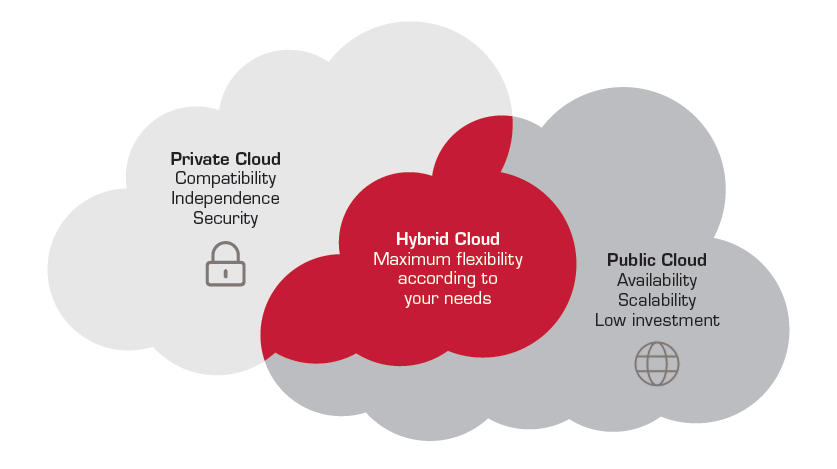
\includegraphics[width=400]{bachproef/img/hybridCloud.png}}
\caption{\textit{Hybrid cloud figuur \autocite{Boris2020hybrid}}}
\label{fig}
\end{figure}
\newpage
\subsection{Service Models}
\label{sec:Service models}

Zoals men eerder schreef wordt cloud computing gevormd door de vijf hiervoor genoemde en beschreven karakteristieken. Verder ook door de vier \textbf{deployment models} waar net over verteld werd en nog drie andere \textbf{service models} waar nu naar gekeken zal worden. deze bestaan namelijk uit:

\begin{itemize}
    \item Software as a Service (SaaS)
    \item Platform as a Service (PaaS)
    \item Infrastructure as a Service (IaaS)
    %\item Network as a Service (NaaS)
\end{itemize}


\subsubsection{SaaS}
\textit{SaaS} is één van de vormen van \textbf{service models} waar de cloud provider applicaties ontwikkelt, onderhoud en deze ter beschikking stelt aan de gebruiker in de vorm van een \textbf{\textit{pay as you go}} model zoals eerder besproken. De cloud provider neemt het hele onderhoudt van de infrastructuur en beveiliging op zich. Via een computer en een internet verbinding kan er gebruik worden gemaakt van de software \autocite{OracleSaaS} \autocite{mell2011nist}.%, een aantal voorbeelden van zulke applicaties zijn bijvoorbeeld:

%\begin{itemize}
%    \item Azure Key Vault \footnote{azure.microsoft.com/nl-nl/services/key-vault}
%    \item AWS Key Management Service \footnote{aws.amazon.com/kms}
%    \item Google Cloud Key Management \footnote{cloud.google.com/security-key-management}
%\end{itemize}

\subsubsection{PaaS}
Bij dit model krijgt de klant de mogelijkheid applicaties te laten lopen op de systemen en ook de keuze om op deze cloud infrastructuur te werken zonder enige zorg aan onderliggende zaken zoals: netwerk, servers, besturing en opslag. Los van deze zaken heeft de gebruiker wel nog altijd autorisatie over de configuraties en beheer van de gelanceerde applicaties en gegevens \autocite{mell2011nist}.

\subsubsection{IaaS}

De mogelijkheid wordt hier voorgesteld bij de gebruiker voor verwerking van data, opslag, netwerken en andere fundamentele computer middelen zodat de gebruiker zelf de keuze heeft om zijn noden te voldoen. De gebruiker beheert de onderliggende cloud infrastructuur niet maar heeft wel controle over de besturing systemen, opslag en gelanceerde applicaties. Verder is er ook de mogelijkheid om de netwerk componenten te configureren voor gelimiteerde toegang \autocite{mell2011nist}.
\newpage
\subsection{Secrets Management als cloud oplossing}
\label{sec:Key managers}
\subsubsection{Azure Key Vault}

Azure Key Vault\footnote{\href{https://azure.microsoft.com/nl-nl/services/key-vault/}{Microsoft Azure Key Vault website}} is een PaaS oplossing dat je toelaat om beveiligd cryptografische sleutels te beheren. Secrets worden onderhouden via deze service. Wanneer bijvoorbeeld, virtuele machines en schijven worden opgezet in de cloud, worden deze door Azure zelf geëncrypteerd. De mogelijkheid is er om zelf een encryptie sleutel te gebruiken om de schijven van virtuele machines te encrypteren. Deze encryptie sleutels kunnen dan via de Azure Key Vault bijgehouden worden. Deze tool laat gecentraliseerd beheer toe voor secrets.

Via het platform kan een secret worden aangemaakt met de kenmerken die eerder werden opgesomd bij het \textit{application-pull} model:

\begin{itemize}
    \item Central management
    \item Access policies
    \item Auditing
    \item Ephemeral credentials
    \item Compartmentalization
    \item Facilitates rotation
\end{itemize}

De secret wordt centraal beheerd via een vault dat kan worden aangemaakt via het Azure platform. Via \textit{Identity Access Management (IAM)} kan er beheerd worden waar een gebruiker toegang tot heeft en welke acties deze gebruiker heeft uitgevoerd \autocite{ganatra2019}. Dit wordt verder ondersteund door het activiteitenlogboek dat Azure aanbiedt binnen de key vault service. Als secrets worden aangemaakt wordt er de keuze gegeven of er een activatie of expiratie moment wordt opgegeven. Dit zorgt er voor dat gegevens vluchtig kunnen zijn. Men kan meerdere vaults maken met meerdere gegevens die voor allerlei applicaties gebruikt worden. Deze worden geleverd aan applicaties via service principals. Dit zijn applicaties dat binnen Azure Active Directory worden aangemaakt om toegang te verkrijgen tot resources in Azure. Deze kunnen gebruikt worden om secrets op te halen voor applicaties. Secrets zijn nooit hard coded en kunnen binnen de key vault opnieuw gegenereerd worden. Deze worden bijgewerkt en applicaties verkrijgen zo geautomatiseerd hun bijgewerkte sleutel. Er zijn meerdere manieren om sleutel generatie en rotatie te automatiseren na een bepaald tijdsinterval. De meest gebruikte manier is via Azure Automation met een geautomatiseerd script \autocite{Majumder2019} \autocite{Marczak2020}.

%Je verwijst bij elke bewering die je doet, vakterm die je introduceert, enz. naar je bronnen. In \LaTeX{} kan dat met het commando \texttt{$\backslash${textcite\{\}}} of \texttt{$\backslash${autocite\{\}}}. Als argument van het commando geef je de ``sleutel'' van een ``record'' in een bibliografische databank in het Bib\LaTeX{}-formaat (een tekstbestand). Als je expliciet naar de auteur verwijst in de zin, gebruik je \texttt{$\backslash${}textcite\{\}}. Soms wil je de auteur niet expliciet vernoemen, dan gebruik je \texttt{$\backslash${}autocite\{\}}. In de volgende paragraaf een voorbeeld van elk.
%%=============================================================================
%% Methodologie
%%=============================================================================

\chapter{\IfLanguageName{dutch}{Methodologie}{Methodology}}
\label{ch:methodologie}

%% TODO: Hoe ben je te werk gegaan? Verdeel je onderzoek in grote fasen, en
%% licht in elke fase toe welke stappen je gevolgd hebt. Verantwoord waarom je
%% op deze manier te werk gegaan bent. Je moet kunnen aantonen dat je de best
%% mogelijke manier toegepast hebt om een antwoord te vinden op de
%% onderzoeksvraag.

In dit hoofdstuk wordt er gekeken naar de mogelijke applicaties en wordt een keuze gemaakt aan de hand van de MoSCoW-methode, deze methode gebruiken we om de kenmerken te lijsten in categorieën om sneller in te zien welke kandidaat meer geschikt is. Dit verdelen we onder vier categorieën waaronder:
\begin{itemize}
    \item Must have
    \item Should have
    \item Could have
    \item Won't have
\end{itemize}

\section{Criteria voor keuze tools}
\subsection{Must have}

In dit gedeelte kijken we naar de absolute must bij een applicatie, zo moet de applicatie aan volgende vereisten voldoen:

\begin{itemize}
    \item Application-pull kenmerken
    \item Open-source
    \item GUI aanwezig (met TLS verbinding)
    \item Ondersteuning voor Windows (OS)
    \item Ondersteuning TeamCity
\end{itemize}

Er wordt een focus gelegd op een gratis applicatie waar men via een GUI, beveiligd met een TLS verbinding, centraal de secrets kan beheren. Er moet ook een vorm van beleid zijn zodat niet iedereen aan elke gegevens kan. Een integratie met TeamCity is in dit geval belangrijk zodat deze gebruikt kan worden bij de proof of concept. Verder is het ook belangrijk binnen Wolters Kluwer dat het centrale platform beveiligd moeten kunnen worden met een getekend certificaat. Dit is een standaard voor platformen binnen het Wolters Kluwer netwerk voor veiligheidsredenen.

\subsection{Should have}

Het zou ook geen te ingewikkeld proces mogen zijn om de opstelling te maken. Dit moet evident op te zetten zijn zodat later andere mensen hiermee zonder veel moeite mee kunnen werken.

\subsection{Could have}

Een integratie met LDAP zodat het secret management systeem met active directory gegevens werkt is een pluspunt. Hiermee wordt er de mogelijkheid gegeven om via \textit{active directory user accounts}, binnen het domein van Wolters Kluweren, authenticatie te verrichten. In een bedrijf zoals Wolters Kluwer wordt LDAP gebruikt wanneer er integraties mogelijk zijn met applicaties. 

\subsection{Won't have}

Een volle integratie met verscheidene applicaties zal niet aan bod komen maar voor de concrete use case met TeamCity wel. Men gaat geen complexe configuraties uitvoeren om alle functionaliteiten te gebruiken.

\section{Keuze tools}

\subsection{On-premise}

\begin{itemize}
    \item Vault
    \item Knox
    \item Confidant
    \item 1Password Secrets Automation
\end{itemize}

\subsubsection{Vault}

Vault\footnote{\href{https://www.vaultproject.io/}{Vault website}} is een secrets management applicatie die in deel \ref{sec:Hashicorp vault} eerder besproken werd. Los van alle technische vereisten waar alle specificaties van komen wordt vault ook voor Windows ondersteund en gebruikt een duidelijke web interface. Vault maakt gebruik van een persistente backend om geëncrypteerde data in te behouden. Hiervoor kan Consul \footnote{\href{https://www.consul.io/}{Consul website}} gebruikt worden. Bij een opstelling zou er voor een simpele backend gekozen worden zoals een lokaal filesystem storage backend. Vault is open source en kan als een managed vault via cloud geleverd worden. TeamCity heeft één plugin \footnote{\href{https://plugins.jetbrains.com/plugin/10011-hashicorp-vault-support}{JetBrains website met Hashicorp Vault plugin}} voor een integratie met Vault dat gebruikt kan worden. Verder is er ook de mogelijkheid voor LDAP te integreren met Vault, zo kunnen AD gebruikers zich aanmelden via de web interface en volgens policies gegevens beheren. 

\subsubsection{Knox}

Knox \footnote{\href{https://github.com/pinterest/knox}{Knox github pagina}} is een applicatie aangemaakt door Pinterest omdat ze problemen hadden met het juist beheren van secrets. Zo bewaarden ze vroeger secrets in source control. Dit zorgde uiteraard voor een secret sprawl. De groei van het aantal ontwikkelaars zorgde ook voor bijkomende risico's zoals malware en phishing indien gegevens lekten. Knox zorgt voor een centraal beheer van secrets. Het geeft de mogelijkheid gebruikers toegang te verlenen wanneer secrets nodig zijn en het systeem ondersteunt de mogelijkheid voor rotatie van de gegevens. Er wordt ook bijgehouden wie welke gegevens gebruikt heeft aan de hand van audit. Knox kan in zowel Linux als MacOS en Windows omgeving worden opgezet samen met de installatie van \textit{GO}\footnote{\href{https://golang.org/doc/install}{GO website}}, de taal waar Knox mee geschreven is. Knox zal ook gebruik moeten maken van een backend. Standaard maakt deze gebruik van een \textit{TempDB} die in geheugen alle data zal opslaan. Maar dit is geen werkwijze om permanent te behouden. Zou de machine uitvallen is alle data verloren. Voor de Backend wordt MySQL, PostgreSQL of sqlite aangeraden \autocite{Lundberg2021}. Knox heeft verder geen community achter zich die integraties met andere applicaties aanbieden. De algemene setup van deze werking is ook zeer complex en is deze geen goede keuze voor een bedrijf zoals Wolters Kluwer.

\subsubsection{Confidant}

Confidant \footnote{\href{https://lyft.github.io/confidant/}{Confidant github pagina}} is een secret management systeem ontworpen door Lyft. Het wordt gebruikt voor exclusief gebruik binnen een AWS omgeving. Als backend voor deze applicatie wordt een DynamoDB gebruikt wat een AWS databank systeem is. Het opzetten van deze opstelling is heel technisch en kan alleen worden gedaan binnen een Docker omgeving of een Linux omgeving. Via Docker kan men deze tool op Windows gebruiken maar er wordt geen gebruik gemaakt van containers. Voor Confidant is er weinig tot geen community die achter het platform staat \autocite{Confidant2021}. 


\subsubsection{1Password Secrets Automation}

1Password Secrets Automation \footnote{\href{https://1password.com/secrets/}{1Password Secrets Automation website}} is een recent uitgekomen secret management system gemaakt door AgileBits Inc die beter bekend staan als de ontwikkelaars van 1Password. In 2021 hebben ze een grote stap gezet door SecretHub\footnote{\href{https://secrethub.io/}{SecretHub website}} aan te kopen waarmee ze hun stap richten naar secrets management \autocite{Schoonen2021}. De tool gebruikt de beveiliging en encryptie mechanismen van 1Password wat een succesvolle tool is die sinds 2006 bestaat. De tool ondersteunt het principe van centraal beheer voor alle secrets met een belang aan audit, key rotation, policy en integraties met reeds bestaande tools \autocite{Shiner2021}. Voor TeamCity is er (nog) geen plugin. Deze tool is ook geen open-source applicatie. Omdat de applicatie bij het schrijven van deze tool vrijwel net uitgekomen is, is er ook niet veel informatie over op het internet bij het gebruik en mogelijke plus, en minpunten.

\subsubsection{Keuze applicatie}

In onderdeel \ref{sec:Hashicorp vault} werd Vault van Hashicorp gebruikt om de uitleg te geven hoe \textit{application-pull} een model is dat zeer sterk secret management definieert. Vault is na veel jaren verder uitgegroeid tot een zeer geschikte applicatie om als secret management system te gebruiken. Deze zal uitgewerkt worden op een Windows systeem.


\subsection{Cloud oplossing}

Wolters Kluwer gebruikt voor het grootste deel Azure als hun cloud solution platform. Hierdoor zal er gekeken worden naar het opzetten en gebruik van Azure Key Vault. Dit is een cloud oplossing die eerder werd besproken en bij Wolters Kluwer al een tijdje interessant leek te zijn om te gebruiken. Juist was er nooit de tijd om hiervoor een project voor op te zetten. Deze zal worden gekozen als cloud oplossing. Voor TeamCity bestaan er enkele plugins die een integratie voeren met Microsoft Azure cloud oplossingen, waaronder één plugin\footnote{\href{https://plugins.jetbrains.com/plugin/11373-azure-key-vault-support}{JetBrains website met Azure Key Vault plugin}} voor Azure Key vault.

\chapter{\IfLanguageName{dutch}{Proof of Concept}{Abstract}}
\label{ch:poc}

In dit hoofdstuk worden de opstellingen met omgevingen voor Hashicorp Vault en Azure Key Vault opgezet. Alle vermelde scripts / playbooks zijn aanwezig op volgende \href{https://github.com/Rayenasr/Secrets-management-thesis}{github repository}\footnote{\href{https://github.com/Rayenasr/Secrets-management-thesis}{github repository}}.

\section{Opzet Hashicorp Vault}

De applicatie wordt opgezet in een virtuele test omgeving, on-premise van het Wolters Kluwer development infrastructuur. Een aantal zaken die aanwezig waren alvorens het begin van de proof of concept (PoC).

\begin{itemize}
    \item Dell laptop binnen het Wolters Kluwer domein met WSL² Ubuntu + ansible 2.10.6  
    \item Virtuele test omgeving binnen Wolters Kluwer domein
    \item API test call script met dank aan de co-promotor
    \item Administrator rechten bij CI/CD tool TeamCity in productie en development
\end{itemize}
\textit{Windows Subsystem for Linux} is een compatibiliteitslaag voor het native draaien van binaire linuxbestanden in een console omgeving op een Windows 10 machine \autocite{wsl2021}. Deze wordt gebruikt om Ansible te laten draaien. Verder zijn de specificaties van de virtuele test omgeving als volgt:

\begin{itemize}
    \item OS: Windows Server 2019 Datacenter (64 bit)
    \item Intel Xeon Silver 4208 CPU @ 2.10GHz
    \item 32GB geheugen
\end{itemize}

\subsection{Installatie \& configuratie Hashicorp Vault}

In onderdeel \ref{ch:ansible}, werd getoond wat Ansible is en hoe deze tool gebruikt wordt om taken te automatiseren. Doorgaans deze PoC zal ansible gebruikt worden voor een aantal taken snel en efficiënt te voltooien. De syntaxis die gebruikt wordt om een Ansible script op te roepen in de WSL² Ubuntu omgeving is als volgt: \textit{ansible-playbook PLAYBOOK.YML -i INVENTORY}. Bij het klaarzetten van de omgeving wordt Ansible gebruikt aan de hand van playbook \href{https://github.com/Rayenasr/Secrets-management-thesis/blob/main/vault/installVault.yml}{\textit{installVault.yml}}\footnote{\href{https://github.com/Rayenasr/Secrets-management-thesis/blob/main/vault/installVault.yml}{installVault.yml op github}} met bijbehorende \href{https://github.com/Rayenasr/Secrets-management-thesis/blob/main/vault/inventory}{inventory file}\footnote{\href{https://github.com/Rayenasr/Secrets-management-thesis/blob/main/vault/inventory}{inventory file op github}}.


\subsubsection{Installatie}
Alvorens het starten, vraagt het playbook om de gebruikersnaam op te geven met bijbehorend wachtwoord. Dit is zo bij elk playbook gedaan zodat we deze gegevens niet rechtstreeks in de inventory file zetten zoals er afgebeeld werd op figuur \ref{fig:inventorypass}. Eens het playbook afgerond is, kan vault opgestart worden via een elevated command prompt. Dit is een command prompt met administrator rechten. De working directory moet dezelfde zijn als de locatie waar \textit{vault.exe} staat. Eens in deze locatie wordt de commando \textit{vault server -config=.\symbol{92}config\symbol{92}config.hcl} gebruikt om vault op te starten met bijbehorende configuratie bestand. 

\begin{figure}[hbtp]
    \caption{inhoud initieel configuratie bestand}
    %\label{code.1}
    \begin{lstlisting}[language=yaml,frame=single]
1.    ui = true
2.    disable_mlock = true
3.    storage "file" {
4.    path = "./data"
5.    }
6.    listener "tcp" {
7.    address     = "0.0.0.0:8200"
8.    tls_disable = "true"
9.    }
10.   api_addr = "http://127.0.0.1:8200"
11.   #cluster_addr = "https://127.0.0.1:8201"
    \end{lstlisting}
\end{figure}
Vault kan worden opgestart in \textit{dev} modus waar de lokale CLI geauthenticeerd is om met vault te communiceren. basis configuraties zijn in deze modus verwerkt en dient als testomgeving. Data wordt (geëncrypteerd) in vluchtige geheugen opgeslagen. Bij het afsluiten van de vault applicatie is alle toegevoegde data verloren. Omdat we bij deze PoC data willen opslaan en de vault omgeving geregeld afgesloten moet worden, is hier gekozen voor een simpel bestandssysteem. In het configuratiebestand wordt dit vermeld. Vault zal de backend bestanden lokaal creëren en encrypteren. Elke keer wanneer men de vault wilt opstarten zal deze in een sealed state zijn. Wanneer vault sealed is verwacht hij de master key om encryptie uit te voeren. Wanneer men de webpagina \textbf{http://127.0.0.1:8200} voor de eerste keer bezoekt, wordt een pagina weergeven om de master key op te delen in een aantal key shares. Verder wordt er ook opgegeven hoeveel key shares er nodig zijn om vault te openen. Deze key shares vormen het vermogen om de master key terug op te bouwen. Bij deze PoC kiezen we voor vijf key shares met drie nodige keys om de master key terug op te bouwen en de vault te openen. Vervolgens kan men een JSON bestand downloaden waar de vijf key shares in staan met een root token. Dit bestand moet zeer goed worden bewaard. Deze key shares zijn nodig om vault te openen wanneer deze sealed is. Indien deze key shares verloren gaan kan men vault op geen andere manier meer openen en is de data verloren! De bijbehorende root token wordt gebruikt om als root gebruiker te authenticeren. Dit is in het begin nodig om policies en gebruikers aan te maken. Verder moet het gebruik van de root key in een productieomgeving tot een minimum gehouden worden.

\begin{figure}[htbp]
\centerline{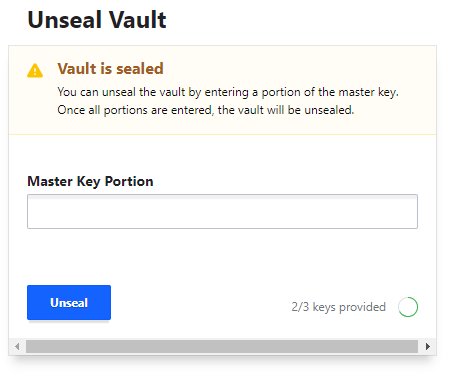
\includegraphics[width=300]{bachproef/img/poc/unsealVault.png}}
\caption{proces om sealed vault te openen \autocite{vault}}
\end{figure}

\subsubsection{Configuratie}
\label{ch:config}

De root key wordt gebruikt om men aan te melden als root gebruiker. Nu men aangemeld is op vault kan men operaties verrichten binnen dit systeem. Hier worden in de volgende delen configuraties verricht:
\begin{itemize}
    \item Secrets (Secrets Engines)
    \item Policies (ACL Policies)
    \item Access (Authentication Methods)
\end{itemize}

Allereerst wordt een nieuwe \textit{secrets engine} aangemaakt. Een secrets engine is een component die data opslaat, encrypteert of decrypteert. Hier wordt er gekozen voor een kv secrets engine aan te maken. Alle standaard waarden worden behouden. Eens deze engine aangemaakt is, kan men hier secrets opslaan met een key-value methode. Hier maken we een secret aan waar we later key-value gegevens aan toe voegen. Deze geven we de naam \textit{TeamCity}. Hierin worden twee secrets aangemaakt, namelijk de keys \textit{TeamCityAccount} en \textit{TeamCityAccountEncryptedPassword} met bijbehorende waarden.
\newline

Vervolgens worden de policies aangemaakt. Hier worden 2 policies aangemaakt, namelijk \textit{teamcity} en \textit{admin}. Dit wordt verricht door een ACL policy aan te maken. Om dit te doen kunnen we via de web ui een policy definiëren. Deze kan ook worden opgeladen. Via ansible laten we het playbook \href{https://github.com/Rayenasr/Secrets-management-thesis/blob/main/vault/createPolicyFiles.yml}{createPolicyFiles.yml}\footnote{\href{https://github.com/Rayenasr/Secrets-management-thesis/blob/main/vault/createPolicyFiles.yml}{createPolicyFiles.yml op github}} lopen om twee HCL bestanden aan te maken waar de policies voor de beide rollen in gedefinieerd staan. Deze worden in de plugin directory gestoken. Voor admin wordt de naam \textit{admin} opgegeven en bijbehorende HCL bestand wordt hierbij opgeladen. Ditzelfde gebeurt ook voor de teamcity policy met naam \textit{teamcity}.

\begin{figure}[htbp]
\centerline{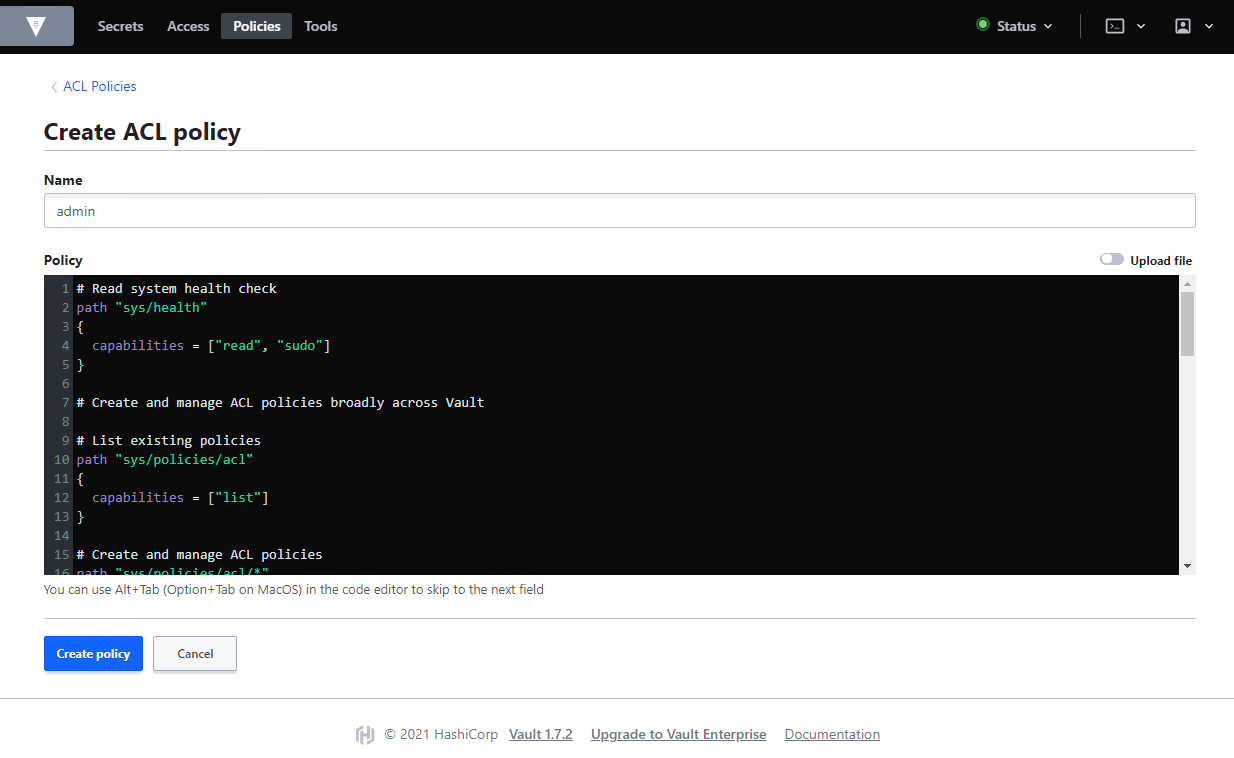
\includegraphics[width=400]{bachproef/img/poc/acl policy.png}}
\caption{proces voor policy aan te maken \autocite{vault}}
\end{figure}

Nu wordt er gekeken naar de access tab. Hier kan men methodes toevoegen om authenticatie te verrichten. Men kan een \textit{userPass} authenticatie methode toevoegen om met gedefinieerde gebruikersnamen met bijbehorende wachtwoorden, aan te melden op het systeem. Dit zal hier niet worden gedaan omdat in deel \ref{ch:ldap} een integratie wordt uitgevoerd met LDAP om AD gegevens te gebruiken binnen het domein van Wolters Kluwer. Er wordt nu wel al een \textit{Approle} toegevoegd. Deze dient als authenticatie methode voor applicaties onder een bepaalde rol. Deze rol wordt aangemaakt zodat via de TeamCity integratie, later secrets kunnen worden opgehaald vanuit vault. De configuratie hiervoor wordt via de CLI van de vault UI uitgevoerd. De configuratie wordt weergeven met output waarden in figuur \ref{ch:role}. Van deze waarden worden later de role\_id en secret\_id values gebruikt voor de plugin integratie met TeamCity.
\newpage


\begin{figure}[htbp]
\centerline{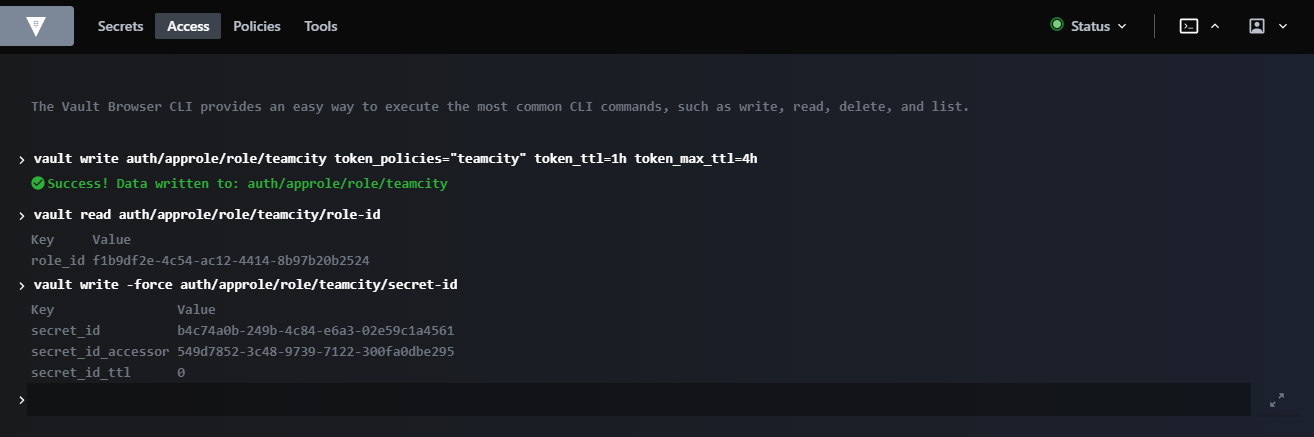
\includegraphics[width=500]{bachproef/img/poc/approle aanmaken.png}}
\caption{proces voor approle aan te maken \autocite{vault}}
\label{ch:role}
\end{figure}

\subsection{LDAP integratie}
\label{ch:ldap}

In een vorig onderdeel werd er gesproken over de access tab waar authenticatie methodes worden toegevoegd. Nu wordt vault geïntegreerd met LDAP zodat gebruikers van het development team zich kunnen verbinden met vault als een gebruiker. Er wordt gekozen voor een nieuwe authenticatie methode. Hier wordt LDAP gekozen. De standaard waarden worden behouden en de methode wordt geactiveerd. Vervolgens komt de configuratie om vault met LDAP te verbinden. Hier wordt de URL gegeven van de domeincontroller: \textit{ldap://EXAMPLE.local:389}. Vervolgens wordt bij User Attribute de waarde \textit{samaccountname} gegeven. Zo kunnen gebruikers via hun gebruikersnaam aanmelden die ze gewoon zijn, bijvoorbeeld \textit{John.Doe}. Vervolgens wordt het bindDn gegeven waarmee gebruikers opgezocht worden \textit{CN=EXAMPLE-IT-LDAP,OU=Service Accounts,OU=EXAMPLE,DC=DC-EXAMPLE} en de userDn \textit{DC=DC-EXAMPLE} met bijbehorende bindpass. Eens dit gelukt is kunnen gebruikers van Wolters Kluwer een verbinding maken met vault. Nu moet er een groep worden aangemaakt waar gebruikers aan toegevoegd worden voor admin rechten. Binnen de LDAP authenticatie methode, maakt men een groep aan genaamd \textit{poc users} met de \textit{admin} policy. Vervolgens kunnen gebruikers worden toegevoegd zodat deze de policy verkrijgen.

\begin{figure}[htbp]
\centerline{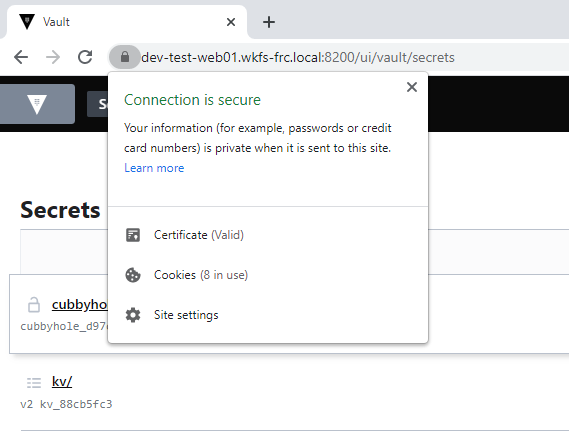
\includegraphics[width=300]{bachproef/img/poc/secure.png}}
\caption{Beveiligde webapplicatie \autocite{vault}}
\label{fig:secure}
\end{figure}
\newpage

\subsection{Installatie SSL certificaat}
In dit onderdeel wordt een SSL certificaat aangemaakt en toegevoegd aan de PoC. Dit is nodig voor het verkeer te beveiligen tussen clients en de vault webpagina. Binnen Wolters Kluwer is dit een requirement om aan te voldoen bij webapplicaties. Om dit te behalen wordt de applicatie \href{https://www.digicert.com/}{\textit{Digicert}\footnote{\href{https://www.digicert.com/}{Digicert website}}} gebruikt. Hiermee wordt een certificaat aanvraag opgesteld die verder behandelt wordt door \textit{Microsoft Active Directory Certificate Services}. Hier wordt de aanvraag verwerkt en verkrijgt men een \textit{certnew.p7b} bestand. Hier is het certificaat in opgeborgen. Daarna gaat men terug naar de Digicert applicatie en wordt dit bestand geïmporteerd. Hieruit kan men vervolgens drie bestanden downloaden. Een \textit{CAcert.crt} bestand en twee andere bestanden behorende tot de host waarvoor de certificaten getekend zijn. In dit geval is dat \textit{dev-test-web01\_wkfs\_local.crt} en \textit{dev-test-web01\_wkfs-frc\_local.key}. Deze drie bestanden worden in de map \textit{certs} gestoken onder \textit{config}. In het configuratie bestand moet er worden verwezen naar deze certificaten. TLS moet ook worden geactiveerd. Het adres \textbf{http://127.0.0.1:8200} zou ook niet meer gebruikt worden, het FQDN \textbf{https://dev-test-web01.wkfs-frc.local:8200} zal hier gebruikt worden. Vervolgens moet de omgevingsvariabele in het systeem ook verandert worden zodat deze ook het juiste adres zal gebruiken. Dit wordt allemaal behaald via het playbook \href{https://github.com/Rayenasr/Secrets-management-thesis/blob/main/vault/updateConfigFile.yml}{updateConfigFile.yml}\footnote{\href{https://github.com/Rayenasr/Secrets-management-thesis/blob/main/vault/updateConfigFile.yml}{updateConfigFile.yml op github}}. Eens het configuratie bestand is bijgewerkt wordt vault opnieuw opgestart om deze te gebruiken. In figuur \ref{fig:ssl} kan men het proces bekijken hoe het resultaat van \ref{fig:secure} behaald werd. 


\begin{figure}
    \centering
    \subfigure[]{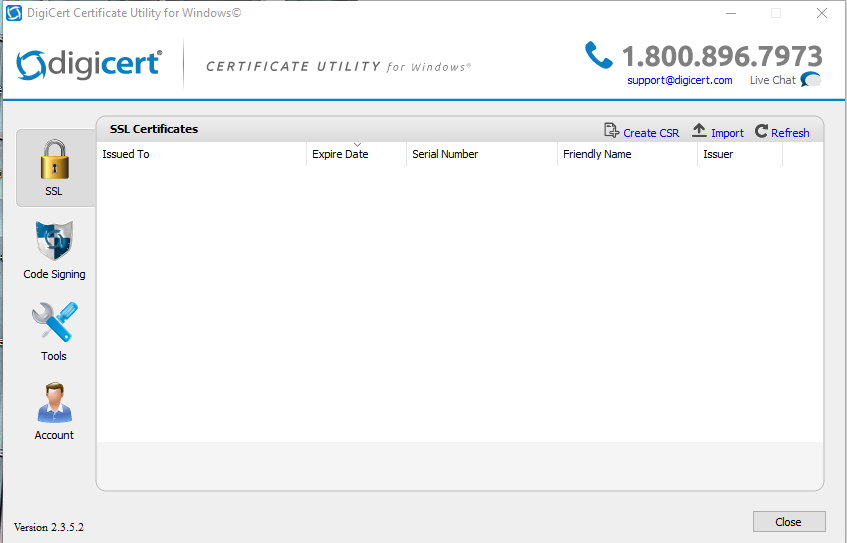
\includegraphics[width=0.4\textwidth]{bachproef/img/poc/digicert.png}}
    \subfigure[]{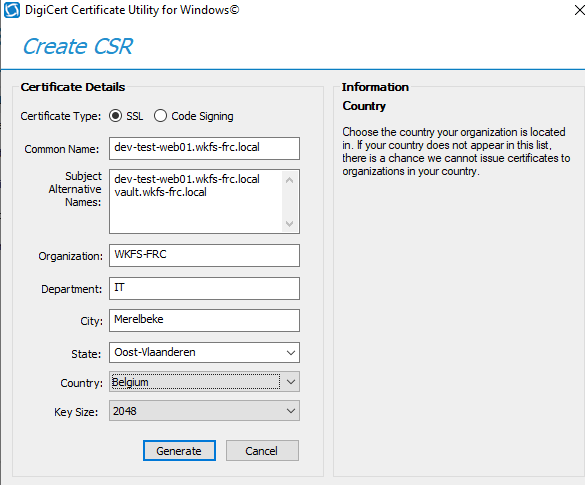
\includegraphics[width=0.4\textwidth]{bachproef/img/poc/1ssl.png}} 
    \subfigure[]{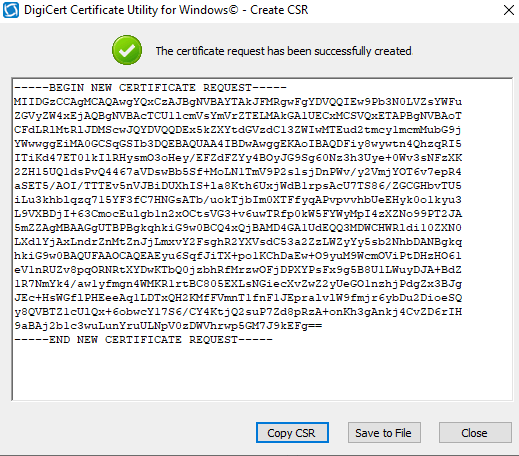
\includegraphics[width=0.4\textwidth]{bachproef/img/poc/2ssl.png}} 
    \subfigure[]{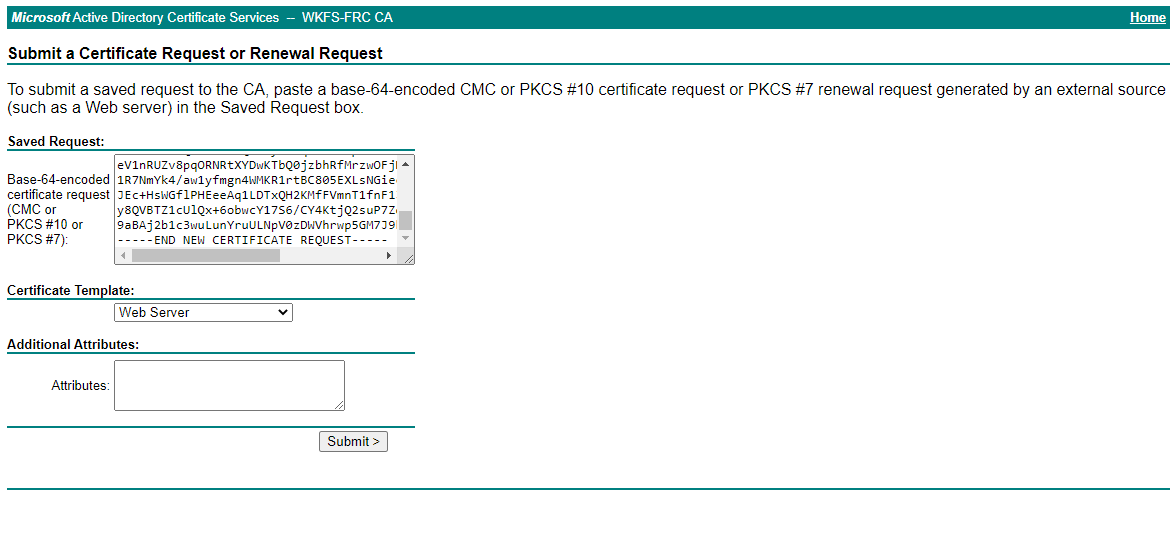
\includegraphics[width=0.4\textwidth]{bachproef/img/poc/3ssl.png}}
    \subfigure[]{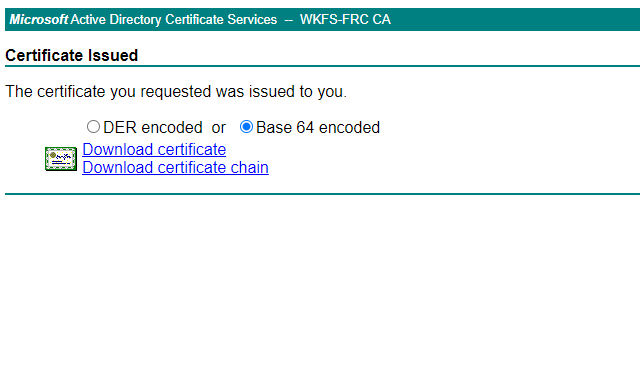
\includegraphics[width=0.4\textwidth]{bachproef/img/poc/4ssl.png}}
    \subfigure[]{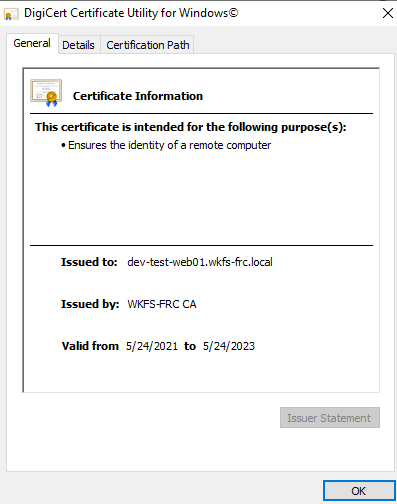
\includegraphics[width=0.4\textwidth]{bachproef/img/poc/5ssl.png}}
    \caption{proces om SSL certificaat te tekenen \autocite{digicert}}
    \label{fig:ssl}
\end{figure}

\newpage
\section{Opzet Azure Key Vault}
\label{ch:azurekey}

Het opzetten van een Key Vault van Azure is minder complex dan een on-premise secrets management opstelling zoals bij Hashicorp Vault. Toch zijn er enkele stappen die uitgevoerd moeten worden voor secrets beheerd kunnen worden. Als eerste wordt een nieuwe resource group aangemaakt. Deze krijgt de naam \textit{rg-devsup-keyvault}. Hier maken we een nieuwe resource. We kiezen voor key vault en noemen deze \textit{kv-devsup}. De recent aangemaakte resource group wordt hier gekozen en de resterende opties worden niet gewijzigd. Hiermee bekomen we tot het resultaat afgebeeld in figuur \ref{fig:azure}.

Vervolgens wordt een \textit{service principal} aangemaakt voor de key vault die gebruikt zal worden door de integratie plugin van Azure Key Vault en TeamCity. Dit wordt behaald via de Azure CLI met commando \textit{az ad sp create-for-rbac --name TeamCityVault}. Vervolgens moeten we enkele waarden verkrijgen over deze service principal die later nodig zijn bij de integratie. Via volgende commando's wordt dit behaald: \textit{az account show --query '{tenantId:tenantId,subscriptionid:id}';} en \textit{az ad sp list --display-name TeamCityVault --query '{clientId:[0].appId}'}. Deze commando's werden door een persoon verricht met bevoegdheden aan Azure AD binnen het Wolters Kluwer domein. De aangemaakte service principal wordt juist nog toegevoegd bij de gebruikers van de key vault. Dit gebeurt via de access policies tab binnen de \textit{kv-devsup} key vault. Dit staat ook afgebeeld op figuur \ref{fig:azure}. Hier wordt de service principal \textit{TeamCityVault} gekozen en toegevoegd met de \textbf{GET} key permission. De service principal moet juist de rechten hebben om secrets op te halen. Nu worden twee secrets aangemaakt in deze vault. Net zoals bij Hashicorp Vault, worden de keys \textit{TeamCityAccount} en \textit{TeamCityAccountEncryptedPassword} met bijbehorende waarden toegevoegd.
\begin{figure}[htbp]
\centerline{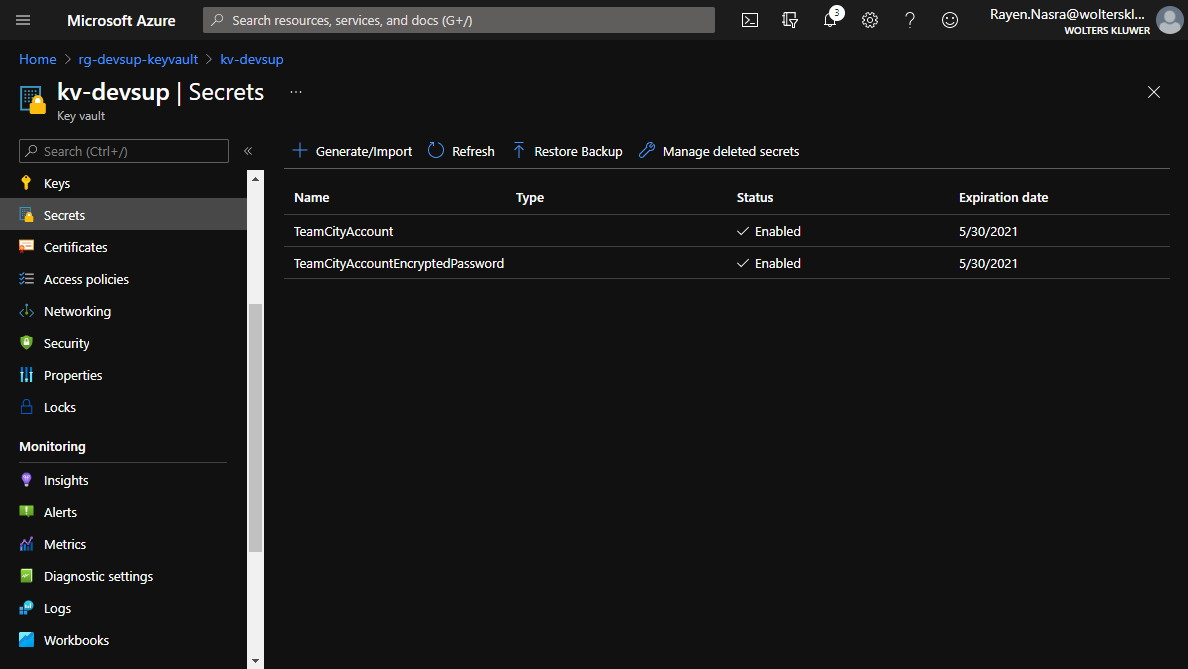
\includegraphics[width=400]{bachproef/img/poc/azurekeyvault.png}}
\caption{Aangemaakte Key Vault in Azure \autocite{azure}}
\label{fig:azure}
\end{figure}

\section{TeamCity omgeving}
\subsection{Integratie tools met TeamCity}

In dit gedeelte worden de integratie plugins geïnstalleerd op TeamCity. Hierna worden connecties vastgelegd met de Azure Key Vault en Hashicorp Vault. Als eerste wordt het playbook \href{https://github.com/Rayenasr/Secrets-management-thesis/blob/main/vault/fetchPlugins.yml}{\textit{fetchPlugins.yml}}\footnote{\href{https://github.com/Rayenasr/Secrets-management-thesis/blob/main/vault/fetchPlugins.yml}{fetchPlugins.yml op github}} gebruikt om de beide plugins te downloaden en klaar te zetten in de vault directory onder \textit{plugins}. Hierna worden deze op de webapplicatie van TeamCity opgeladen via volgende stappen:

\begin{enumerate}
  \item Op het homescreen van TeamCity kiest men voor het tandwiel icoon (Administration)
  \item Nu kiest men voor \textit{plugins} onder \textit{Server Administration}
  \item Hier laad men elke plugin afzonderlijk op
  \item De toegevoegde plugins worden ingeladen en zijn klaar voor gebruik
\end{enumerate}

Er is een project aangemaakt dat dient als test case. Om hier de Azure Key Vault plugin en de Hashicorp Plugin te gebruiken moeten eerst connecties worden vastgelegd. Hier worden de eerder aangemaakte approle van vault, en de service principal van azure voor gebruikt. Dit wordt behaald via volgende stappen:

\begin{enumerate}
  \item Het Secret Management project word gekozen onder \textit{Development Support\symbol{92}Playground\symbol{92}Secret Management}
  \item Hier kiest men voor \textit{edit project settings}
  \item Verder wordt onder \textit{General Settings}, \textit{Connections} gekozen
  \item Hier worden voor zowel Hashicorp Vault als Azure Key Vault een connectie toegevoegd. Voorbeeld bij figuur \ref{fig:connections}
\end{enumerate}

\begin{figure}[!htb]
    \centering
    \subfigure[Azure Key Vault]{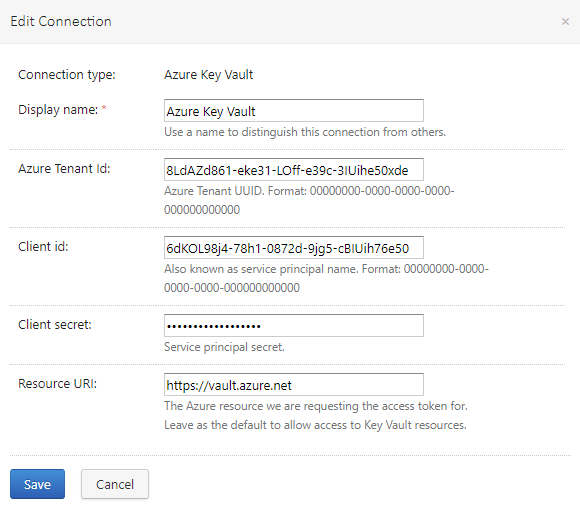
\includegraphics[width=0.4\textwidth]{bachproef/img/poc/KeyVaultConnection.png}}
    \subfigure[Hashicorp Vault]{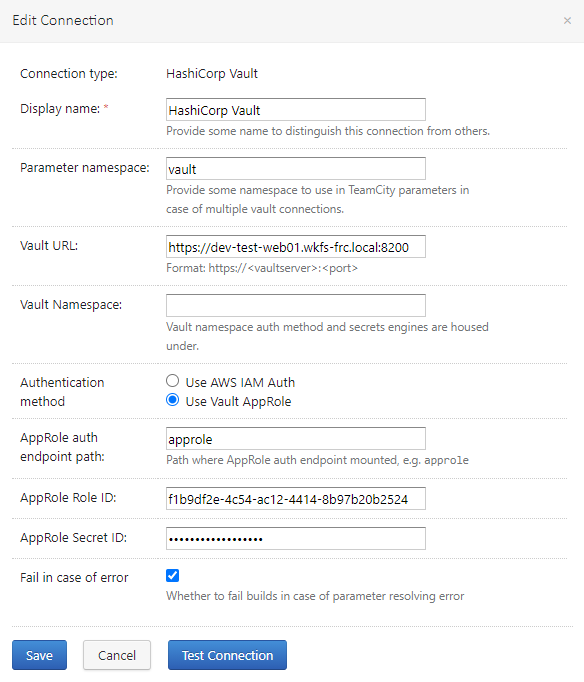
\includegraphics[width=0.4\textwidth]{bachproef/img/poc/VaultConnection.png}} 
    \caption{proces connecties toe te voegen \autocite{teamcity}}
    \label{fig:connections}
\end{figure}

\subsection{Secret Management Project}
In TeamCity is er een project voorzien om meerdere build configuraties aan te maken. Voor Azure Key Vault en Hashicorp Vault worden twee verschillende build configuraties opgesteld onder hetzelfde project. De plugins doen hun werking aan de hand van omgevingsvariabelen die alvorens deployments van builds worden gedeclareerd. De plugins doen hun werking wanneer deze variabelen worden meegegeven als script argumenten. Hierdoor worden deze opgehaald en toegevoegd aan het proces van de build. Dit wordt behaald onder de configuratie opties van het project, onder \textit{parameters}. Omgevingsvariabelen worden gedeclareerd met het prefix `\textit{.env}`. Zo kan een variabele met naam \textit{env.AgentsAmount} worden aangemaakt met een vaste waarde. Voor de Hashicorp Vault plugin geldt volgende syntaxis `\textbf{\%vault:PATH!KEY\%}`. Voor Azure key vault is dat `\textbf{\%keyvault:VAULT NAME/SECRET NAME\%}`. De waarden waar naar gerefereerd moet worden zijn de waarden die in deel \ref{ch:config} reeds toegevoegd zijn geweest bij hashicorp vault. Voor azure key vault werd dit gedaan in deel \ref{ch:azurekey}. Op figuur \ref{fig:envvar} staan voorbeelden waar deze variabelen worden toegevoegd.
%Volgende variabelen worden toegevoegd voor de hashicorp vault build: \textit{env.TeamCityAccount} met waarde\textit{\%vault:kv/TeamCity!/TeamCityAccount\%}, vervolgens variabele  \textit{env.TeamCityAccountEncryptedPassword} met waarde \textit{\%vault:kv/TeamCity!/TeamCityAccountEncryptedPassword2\%} toegevoegd. 

%Het formaat voor de azure key vault variabele is als volgt \textbf{\%keyvault:<vault name>/<secret name>\%}. Hiermee worden in de andere configuratie build volgende omgevingsvariabelen opgegeven: \textit{env.TeamCityAccount} met waarde \textit{\%keyvault:kv-devsup/TeamCityAccount\%}, vervolgens variabele \textit{env.TeamCityAccountEncryptedPassword} met waarde \textit{\%keyvault:kv-devsup/TeamCityAccountEncryptedPassword\%} 

\begin{figure}[!htb]
    \centering
    \subfigure[Azure Key Vault]{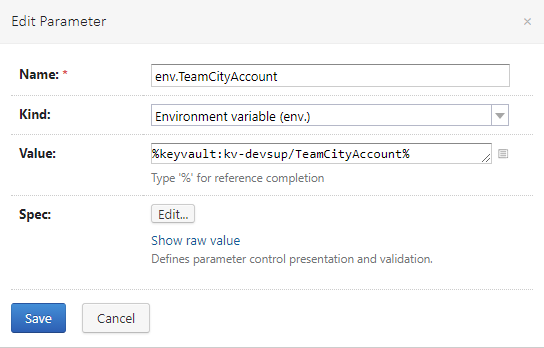
\includegraphics[width=0.45\textwidth]{bachproef/img/poc/AzureParam.png}}
    \subfigure[Hashicorp Vault]{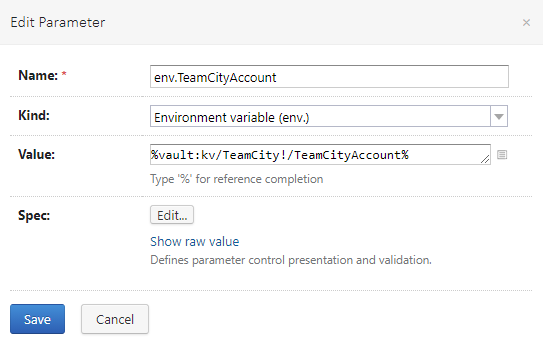
\includegraphics[width=0.45\textwidth]{bachproef/img/poc/VaultParam.png}} 
    \subfigure[Azure Key Vault]{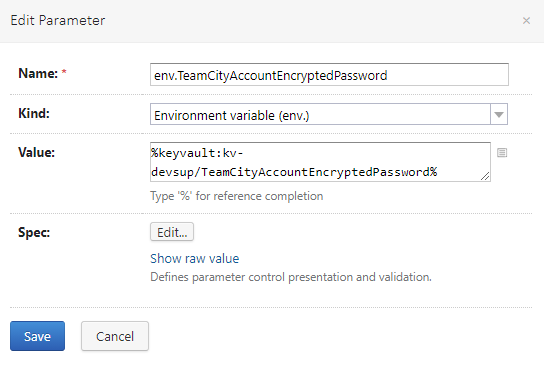
\includegraphics[width=0.45\textwidth]{bachproef/img/poc/AzureParam2.png}}
    \subfigure[Hashicorp Vault]{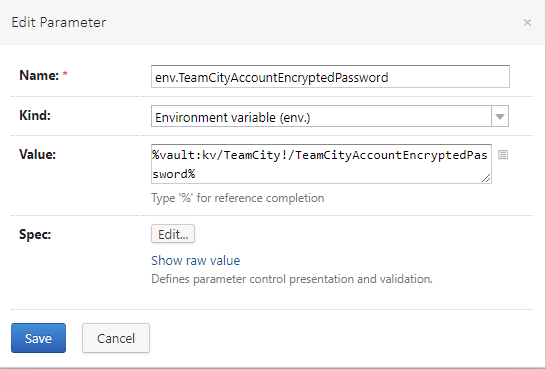
\includegraphics[width=0.45\textwidth]{bachproef/img/poc/VaultParam2.png}} 
    \caption{omgevingsvariabelen toevoegen \autocite{teamcity}}
    \label{fig:envvar}
\end{figure}
\newpage
Voor beide build configuraties worden dezelfde build steps aangemaakt. Hier wordt een powershell script \href{https://github.com/Rayenasr/Secrets-management-thesis/blob/main/TeamCity/RunJobWithVault.ps1}{RunJobWithVault.ps1}\footnote{\href{https://github.com/Rayenasr/Secrets-management-thesis/blob/main/TeamCity/RunJobWithVault.ps1}{RunJobWithVault.ps1 op github}} opgeroepen waar de omgevingsvariabelen meegegeven worden. Deze worden toegevoegd aan het \textit{Scrip argument} gedeelte als ``\textbf{"\%env.TeamCityAccount\%"}`` en ``\textbf{"\%env.TeamCityAccountEncryptedPassword\%"}``. Dit is het gedeelte waar de plugins de syntaxis van de variabelen zullen opmerken eens deze opgeroepen worden bij builds. Deze gegevens kunnen worden opgeslagen en verborgen gehouden in het TeamCity systeem waar ze gemaskeerd worden. Deze worden dus niet geëncrypteerd. In deze instantie worden de waarden geleverd door de vaults van Hashicorp en Azure. Dit voegt een extra abstractielaag tussen TeamCity en gebruikte secrets. Wanneer een build wordt opgeroepen wordt een bepaalde agent die inactief is, verwezen om de uitvoering te doen. Bij deze build wordt het script opgeroepen vanuit een netwerkshare en worden de omgevingsvariabelen meegegeven. Het script zal ervoor zorgen dat een API call naar de TeamCity server wordt gemaakt met gegevens van een administrator, waarmee een andere build wordt gestart. Deze tweede build heeft als enige werking een output te geven met de gebruikte secrets van de vorige build. Met andere woorden worden in beide scripts de secrets opgeroepen. In het tweede script wilt hij deze dan effectief in de output weergeven.

De werking van de Azure Key Vault build wordt in figuur \ref{fig:azurescripts} afgebeeld. Hier kan men opmerken dat de secrets via de eerder ingestelde connectie worden opgehaald. In de build agent wordt de access token in het vluchtige geheugen opgenomen waarmee toegang wordt aangevraagd aan Azure AD, gelimiteerd tot de key vault \textit{kv-devsup}. De secrets worden geleverd als een wachtwoord parameter. De TeamCity server heeft nooit toegang tot de secrets en deze operaties worden meten gedelegeerd aan de build agent. \autocite{azurekvplug}

\begin{figure}[!htb]
    \centering
    \subfigure[API Call met secrets request]{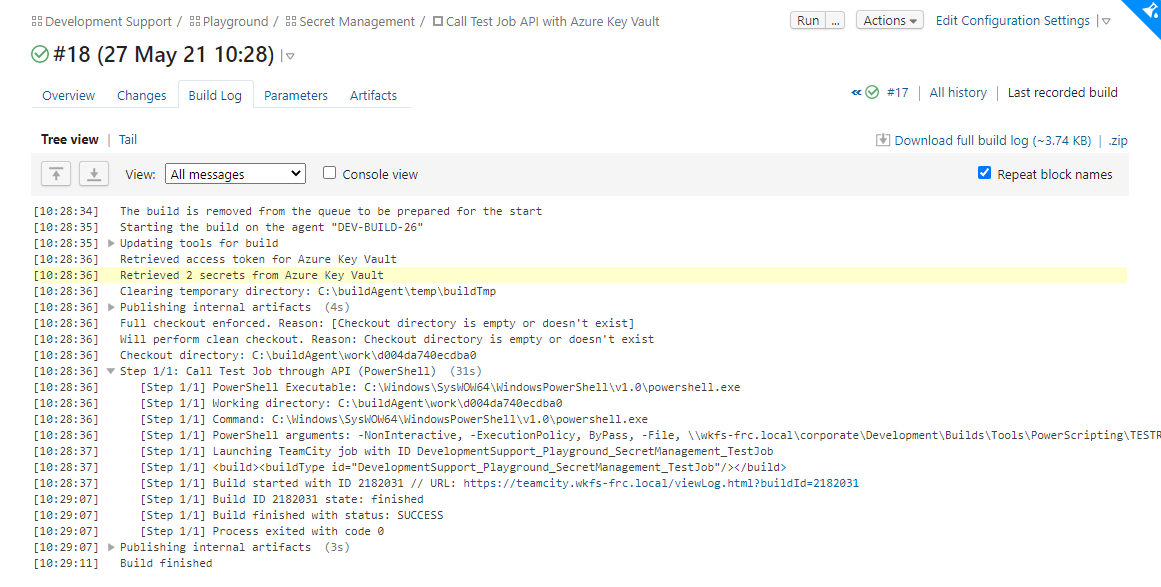
\includegraphics[width=1\textwidth]{bachproef/img/poc/script1output.png}}
    \subfigure[secrets request en printen hiervan]{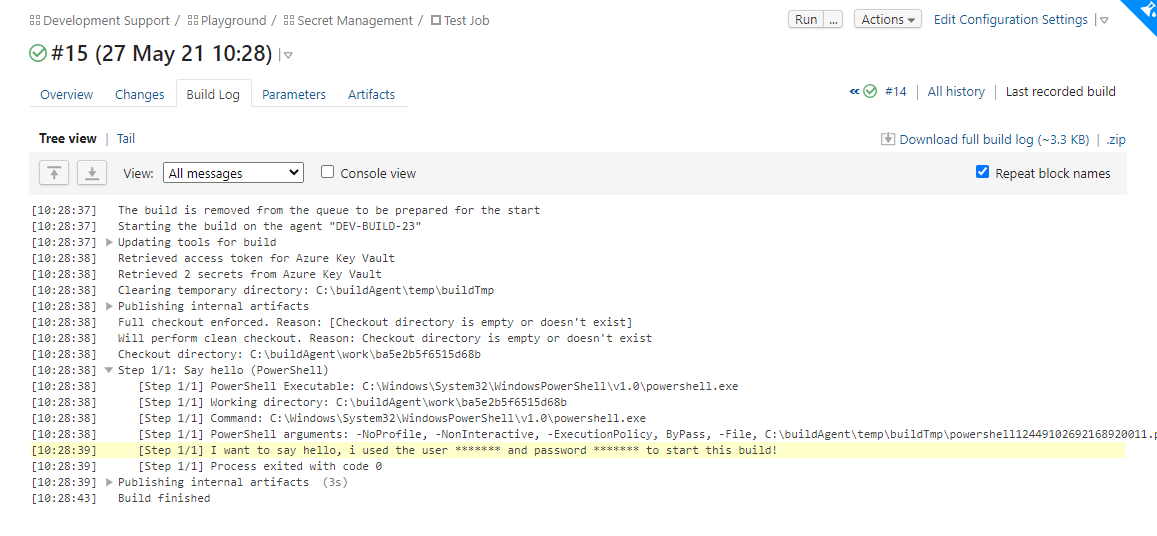
\includegraphics[width=1\textwidth]{bachproef/img/poc/script2output.png}} 
    \caption{Build logs van azure key vault werking \autocite{teamcity}}
    \label{fig:azurescripts}
\end{figure}
\newpage

Voor Hashicorp Vault is deze werking niet gelukt. De configuraties van Vault zijn juist uitgevoerd en de approle is juist ingesteld voor TeamCity waarmee de connectiviteitstest succesvol voltooid, dit wordt afgebeeld in figuur \ref{fig:approlec}. De plugin die gebruikt is faalt om de omgevingsvariabelen op te merken met de nodige gebruikte syntaxis. Waar het probleem bij ligt is niet meteen duidelijk maar het is wel duidelijk dat bij de builds geen logboekvermeldingen komen in verband met de Hashicorp Vault Plugin. Deze testen zijn gebeurt op zowel Windows als Linux agents en twee instanties van TeamCity. Als laatste wordt er in figuur \ref{fig:project} het secrets management project afgebeeld met lopende builds.

\begin{figure}[htbp]
\centerline{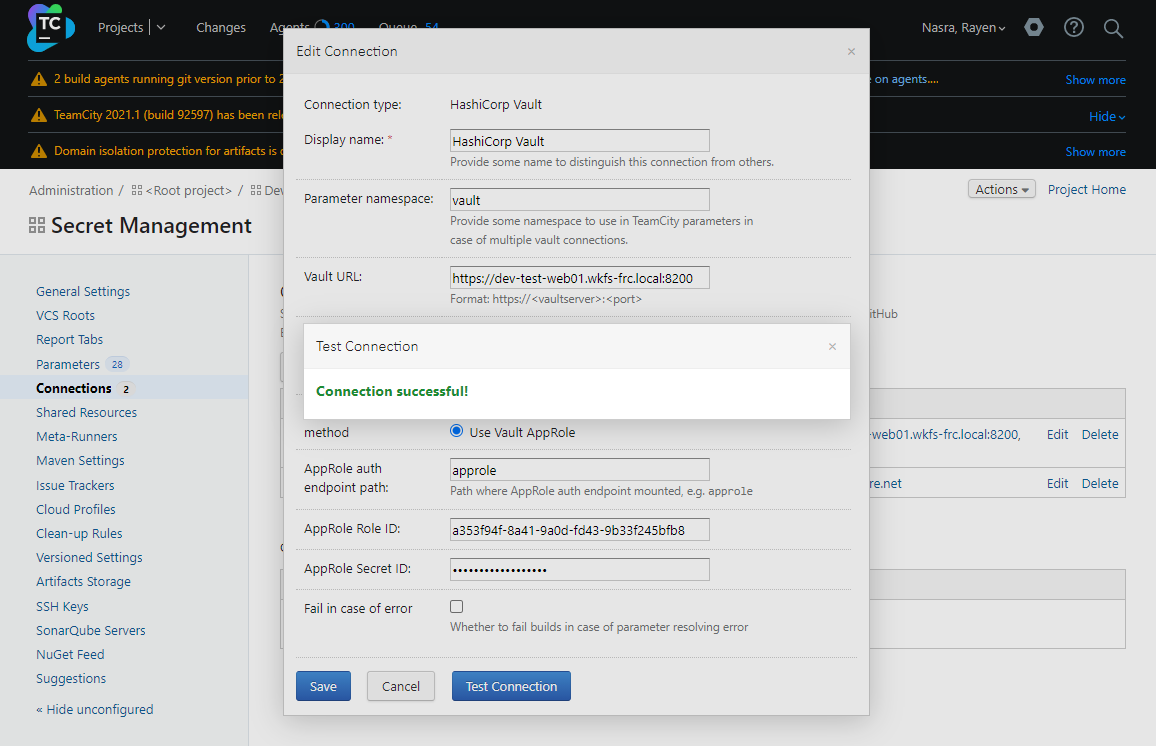
\includegraphics[width=300]{bachproef/img/poc/test connection.png}}
\caption{Connectiviteitstest TLS verbinding in WK domein, met approle TeamCity \autocite{teamcity}}
\label{fig:approlec}
\end{figure}

\begin{figure}[htbp]
\centerline{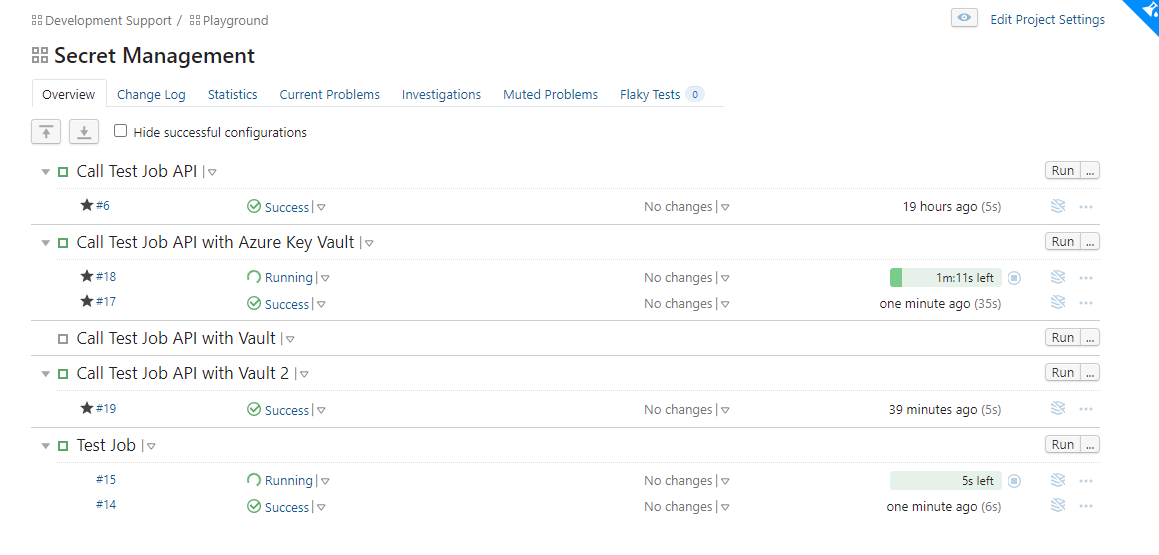
\includegraphics[width=400]{bachproef/img/poc/lopendebuilds.png}}
\caption{Secrets Management project in TeamCity met lopende builds \autocite{teamcity}}
\label{fig:project}
\end{figure}
% Voeg hier je eigen hoofdstukken toe die de ``corpus'' van je bachelorproef
% vormen. De structuur en titels hangen af van je eigen onderzoek. Je kan bv.
% elke fase in je onderzoek in een apart hoofdstuk bespreken.

%\input{...}
%\input{...}
%...

%%=============================================================================
%% Conclusie
%%=============================================================================

\chapter{Conclusie}
\label{ch:conclusie}

% TODO: Trek een duidelijke conclusie, in de vorm van een antwoord op de
% onderzoeksvra(a)g(en). Wat was jouw bijdrage aan het onderzoeksdomein en
% hoe biedt dit meerwaarde aan het vakgebied/doelgroep? 
% Reflecteer kritisch over het resultaat. In Engelse teksten wordt deze sectie
% ``Discussion'' genoemd. Had je deze uitkomst verwacht? Zijn er zaken die nog
% niet duidelijk zijn?
% Heeft het onderzoek geleid tot nieuwe vragen die uitnodigen tot verder 
%onderzoek?


Na het onderzoek kunnen we concluderen dat secrets management systemen zeker gebruikt kunnen worden bij automatiseren wanneer gevoelige data gebruikt wordt. Een complexe hiërarchie van secrets behouden voor elke automatisering tool, afzonderlijk van elkaar, is een zeer lastige taak. Bij aanvang van deze proef werden enkele onderzoeksvragen opgesteld, waar doorheen deze proef een antwoord op werd gezocht. Deze onderzoeksvragen zijn als volgt: `` Welke open-source applicatie kan er gebruikt worden om \textbf{secrets} te beheren? ``, `` Welke cloud oplossing kan er gebruikt worden om \textbf{secrets} te beheren? `` en `` Welke opstelling on-premise of via cloud oplossing, geeft een betere werking voor de use case met TeamCity? ``.

Op de onderzoeksvraag `` Welke open-source applicatie kan er gebruikt worden om \textbf{secrets} te beheren? ``, was Hashicorp Vault de meest interessante tool. De MoSCoW-methode werd gehanteerd om gelijkaardige tools te vergelijken op basis van een aantal kenmerken. Hashicorp Vault is ook de tool waarmee mijn interesse gewekt werd naar dit onderwerp. Het is een breed systeem die over de jaren heen de uitdagingen aanging die secret management aankaart. Voor de tweede onderzoeksvraag `` Welke cloud oplossing kan er gebruikt worden om \textbf{secrets} te beheren? `` werd de tool Azure Key Vault gekozen omdat Wolters Kluwer grotendeels Azure Cloud oplossingen hanteert. Bij Azure Key Vault lag ook meer de voorkeur voor gemak aan integratie door middel van zaken zoals Azure AD dat reeds gebruikt werd. 

Van dit onderzoek werd verwacht dat de opstellingen niet te complex zouden zijn om op te zetten en voor Azure Key Vault was dit inderdaad het geval. Door het feit dat dit een cloud oplossing is, worden de stappen om deze te gebruiken, zo gebruiksvriendelijk mogelijk gehouden. Hier schuilen nog altijd technische competenties achter. Bij Hashicorp Vault was het opzetten iets meer complex door de reden dat deze volledig on-premise was. Een LDAP integratie samen met een SSL certificering zet deze opstelling goed om direct gebruikt te worden door het development team. Enige verdere integraties met andere applicaties kunnen dan ook verwezenlijkt worden. 

Op de laatste onderzoeksvraag `` Welke opstelling on premise of via cloud geeft een betere werking voor de use case met TeamCity? `` werd door middel van de proof of concept, een resultaat behaald, ook al is dit niet wat er in eerste instantie verwacht werd. De proof of concept is niet volledig gelukt. De integraties van TeamCity met de plugins van Azure Key Vault en Hashicorp Vault zijn gelukt. Voor Azure Key Vault zijn de test builds die werden opgesteld geslaagd met de juiste \& verwachte werking. Secrets worden aangeroepen vanuit een beveiligde locatie waar deze centraal beheerd worden. Deze gegevens worden tijdelijk gebruikt zonder dat ze op de TeamCity server, noch de agent opgeslagen worden. Voor Hashicorp Vault is deze zelfde werking niet gelukt. De integratie was succesvol voltooid maar secrets worden niet opgeroepen. Na enige troubleshooting zou het probleem boven water kunnen komen. 

Secrets management systemen bevatten veel domeinen die in de proof of concept niet aan bod zijn gekomen. Door de functionaliteiten die ter beschikking gesteld zijn, kan het zeer interessant zijn om deze verder te configureren en integraties te voeren met andere applicaties. Verder kan het ook zeker interessant zijn om deze functionaliteiten in de toekomst verder te onderzoeken.

%%=============================================================================
%% Bijlagen
%%=============================================================================

\appendix
\renewcommand{\chaptername}{Appendix}

%%---------- Onderzoeksvoorstel -----------------------------------------------

\chapter{Onderzoeksvoorstel}

Het onderwerp van deze bachelorproef is gebaseerd op een onderzoeksvoorstel dat vooraf werd beoordeeld door de promotor. Dat voorstel is opgenomen in deze bijlage.

% Verwijzing naar het bestand met de inhoud van het onderzoeksvoorstel
%---------- Inleiding ---------------------------------------------------------

\section{Introductie} % The \section*{} command stops section numbering
\label{sec:introductie}

Het is een herkenbare situatie bij bedrijven wanneer gevoelige data zoals gebruikersnamen en wachtwoorden, extensief gebruikt worden bij automatisatie gebieden. Het probleem hiermee is dat deze gegevens makkelijk verspreid geraken in allerlei bestanden en uiteindelijk terecht komen op \textit{version control} systemen zoals github \footnote{https://github.com} of bitbucket \footnote{https://bitbucket.org}. Deze manier van werken zorgt na een tijd voor een overvloed aan gevoelige data in meerdere locaties, zonder enig idee van wat waar is. Dit noemt men een \textbf{Secret Sprawl} \autocite{Tozzi2020}. Dit is qua beveiliging geen prettige situatie en men weet niet welke personen deze data kunnen bekijken, en of deze personen bevoegd zijn. \textbf{Secret Management} is de term die gebruikt wordt die dit probleem de baas probeert te zijn. Het gaat om een gecentraliseerde locatie waar \textbf{secrets} beheerd en verleend worden aan applicaties en gebruikers die deze nodig hebben om taken uit te voeren \autocite{Hoffman2021}. Dit brengt een niveau van veiligheid en abstractie omhoog terwijl de integratie met applicaties vlot gebeurd.

Dit onderzoek en de opstellingen die worden aangemaakt zijn binnen het kader van het development team binnen \textit{Wolters Kluwer} \footnote{https://www.wolterskluwer.com/nl-be} waar de bruikbaarheid van secrets management bewezen wordt en een integratie wordt uitgevoerd met Teamcity, een CI/CD applicatie. Verder wordt dit proces geautomatiseerd tot waar mogelijk. Hieruit volgen volgende onderzoeksvragen:

%\hspace{1cm}
\begin{itemize}
    \item Welke open-source applicatie kan er gebruikt worden om \textbf{secrets} te beheren?
    \item Welke cloud oplossing kan er gebruikt worden om \textbf{secrets} te beheren?
    \item Welke opstelling on-premise of via cloud oplossing, geeft een betere werking voor de use case met TeamCity?
\end{itemize}

%\begin{itemize}
%  \item de probleemstelling en context
%  \item de motivatie en relevantie voor het onderzoek
%  \item de doelstelling en onderzoeksvraag/-vragen
%\end{itemize}

%---------- Stand van zaken ---------------------------------------------------

\section{State-of-the-art}
\label{sec:state-of-the-art}
\textbf{Secret management} verwijst naar hulpmiddelen en methodes om digitale authenticatie en autorisatie tot systemen te beheren. Dit houdt in dat data zoals sleutels, wachtwoorden, API tokens, bevoegde accounts en dergelijke gevoelige data niet zomaar eindigen in onbewerkte teksten. deze data noemt men \textbf{secrets}. Het gebruik van secrets in meerdere locaties voor bepaalde doeleinden te behalen gaat tegen de beveiligingsnormen die standaard gelden binnen IT maar alsnog geschonden worden. Men weet op deze manier dan ook niet welke gebruikers toegang hebben tot bestanden waar lichtgevoelige data aanwezig is. Hiermee wordt er ook niet bijgehouden in welke locaties al die gevoelige data kan zitten. Via secrets management probeert men dit probleem aan te pakken. Enkele applicaties die het concept van secrets management ondersteunen zijn:

%\hspace{1cm}
\begin{itemize}
    \item Vault
    \item Keywhiz
    \item Confidant
\end{itemize}
%\hspace{1cm}

Volgens de \textbf{Verizon Data Breach report (2020)} waren 77\% van de cloud inbreuken gerelateerd met gecompromitteerde inloggegevens, met andere woorden, \textit{secrets} \autocite{Hoffman2021}. Dit impliceert naar een zwakke focus voor secret management terwijl bedrijven hun beveiliging systemen optimaal proberen te houden. Verder is er ook de vraag of er cloud oplossingen zijn om dit probleem aan te pakken? Maar om dit eerst te verstaan wordt het concept van cloud oplossingen uitgelegd. 

Cloud oplossingen zijn services aangeboden door \textbf{Cloud Service providers} om bepaalde problemen op te lossen via het internet. Gebruikers krijgen computerdiensten die veel positieve kenmerken met zich meeneemt, onder andere:

%\hspace{1cm}
\begin{itemize}
    \item kostenefficiënt
    \item schaalbaarheid
    \item veiligheid van data
    \item flexibiliteit
\end{itemize}
%\hspace{1cm}

Qua kosten-efficiëntie kan er gekeken worden dat er geen geld meer besteed moet worden aan een IT-infrastructuur en hiervoor moet geen locatie voor worden voorzien. De kosten dalen door het feit dat er ook niets meer onderhouden moet worden en niet moet gekeken worden naar opschalen waarbij geen extra apparatuur aangeschaft moet worden. Via een \textit{Cloud Service Provider} kan er makkelijk opgeschaald of afgeschaald worden naargelang de situatie en welke noden er voldaan moeten worden. In vergelijking met zelf een IT-infrastructuur te beheren is hier het grote voordeel dat men juist betaalt voor de functionaliteit van het apparatuur. Deze providers houden hun cybersecurity optimaal en investeren hier veel geld in, zo hebben de klanten altijd hun \textit{Cloud Resources} ter beschikking zonder dat daar omtrent veel zorgen over zijn. Het enige dat vereist wordt bij de klant, is dat er een internetverbinding aanwezig is. Wat tegenwoordig een standaard hoort te zijn. Dergelijke zaken zoals het juist laten werken van de machines en beveiligingsmaatregelen wordt volledig opgenomen door de cloud service provider \autocite{WouterCloudInvest2020}. Om het concept van cloud oplossingen verder te begrijpen wordt er ook uitleg gegeven over de verschillende \textit{Cloud Delivery Models}, namelijk:

%\hspace{1cm}
\begin{itemize}
    \item 'Infrastructure as a Service' (IaaS)
    \item 'Platform as a Service' (PaaS)
    \item 'Software as a Service' (SaaS)
\end{itemize}
%\hspace{1cm}

Bij \textbf{IaaS} wordt het bij een eindgebruiker mogelijk gesteld om rekenkrachten en opslag te huren zonder dat zij zich zorgen moeten maken over onderhoud of kosten om deze servers te laten draaien. Dit stelt voor een eindgebruiker de grootste vrijheid van de 3 modellen. Daarnaast is er ook \textbf{PaaS} Waar de eindgebruiker, hetzij ontwikkelaars, hetzij zakelijke gebruikers, makkelijker en sneller applicaties kunnen ontwikkelen zonder enige zorg om het beheer van de servers. 
Als laatste is er ook \textbf{SaaS}. Bij SaaS wordt een software als online dienst geleverd aan de eindgebruiker \autocite{hurwitz2020cloud}. 

Een bedrijf is zelf verantwoordelijk voor de \textbf{secrets management}, het is anders ook niet logisch dat een service provider voor elke gebruiker de \textbf{secrets} gaat beheren. Soms passeert er wel de term 'Secrets as a Service', maar dit is geen populaire term. Hier is er een service van, genaamd \textbf{AWS IAM}, waar gebruikers zich zelf moeten laten identificeren voor authenticatie te verkrijgen om \textit{secret services} te gebruiken, onder andere toegang tot bepaalde resources \autocite{thoughtworks2019}. Dit is een tool van amazon web services (AWS) om cloud resources op een veilige manier te gebruiken en beheren. Hiermee de volgende vraag of er nog mogelijke cloud oplossingen zijn die een mogelijkheid aanbieden om \textbf{secrets} te beheren? Enkele mogelijkheden zijn:

%\hspace{1cm}
\begin{itemize}
    \item Cloud KMS van Google Cloud \footnote{https://cloud.google.com/security-key-management}
    \item Key Vault van Microsoft Azure \footnote{https://azure.microsoft.com/en-us/services/key-vault/}
    \item AWS Secrets Manager van Amazon Web Services \footnote{https://aws.amazon.com/secrets-manager/}
\end{itemize}
%\hspace{1cm}

Het is interessant om te zien welke applicaties en technieken er tegenwoordig bestaan om \textbf{secrets} zo goed mogelijk te beheren.

%Hier beschrijf je de \emph{state-of-the-art} rondom je gekozen onderzoeksdomein. Dit kan %bijvoorbeeld een literatuurstudie zijn. Je mag de titel van deze sectie ook aanpassen %(literatuurstudie, stand van zaken, enz.). Zijn er al gelijkaardige onderzoeken gevoerd? %Wat concluderen ze? Wat is het verschil met jouw onderzoek? Wat is de relevantie met %jouw onderzoek?

%Verwijs bij elke introductie van een term of bewering over het domein naar de %vakliteratuur, bijvoorbeeld~\autocite{Doll1954}! Denk zeker goed na welke werken je %refereert en waarom.

% Voor literatuurverwijzingen zijn er twee belangrijke commando's:
% \autocite{KEY} => (Auteur, jaartal) Gebruik dit als de naam van de auteur
%   geen onderdeel is van de zin.
% \textcite{KEY} => Auteur (jaartal)  Gebruik dit als de auteursnaam wel een
%   functie heeft in de zin (bv. ``Uit onderzoek door Doll & Hill (1954) bleek
%   ...'')

%Je mag gerust gebruik maken van subsecties in dit onderdeel.

%---------- Methodologie ------------------------------------------------------
\section{Methodologie}
\label{sec:methodologie}

%Voor het onderzoek zullen er enkele vragenlijsten opgesteld worden en enkele interviews gehouden worden. Deze worden ingevuld door verschillende ondernemingen, werknemers alsook werkgevers. die door de covid crisis, een periode in halt zijn moeten gaan en die een interne werking hebben moeten aanpassen door een vorm van cloud oplossing te integreren in het bedrijf. Deze data wordt verzamelt en verwerkt in grafieken waarmee er een visuele verduidelijking is van hoe bedrijven beïnvloed zijn geweest door de covid crisis, of deze een positieve/negatieve draai aan de onderneming heeft gegeven en hoe de visie tegenover de toekomst verandert is.

Om de onderzoeksvragen te kunnen beantwoorden zal er allereerst een literatuurstudie worden uitgevoerd om te weten welke benaderingen er bij \textbf{secret management} werden uitgevoerd en welke applicaties beschikbaar zijn om een \textit{vault} aan te maken voor de \textbf{secrets} mee te beheren, verder wordt onderzocht bij welke applicaties er integratie mogelijkheden zijn met Teamcity \footnote{https://www.jetbrains.com/teamcity}. Deze CI/CD applicatie maakt gebruik van \textit{version control} om aan bepaalde bestanden te komen om applicaties op te bouwen, in deze bestanden eindigen soms belangrijke gegevens die geweerd moeten worden uit dit systeem. Er zal gekeken worden naar mogelijkheden om processen te automatiseren. Er wordt dan vooral gekeken naar een cloud oplossing en een on-premise opstelling. de verschillende tools worden opgezet en dienen het reële probleem op te lossen.

%Hier beschrijf je hoe je van plan bent het onderzoek te voeren. Welke onderzoekstechniek ga je toepassen om elk van je onderzoeksvragen te beantwoorden? Gebruik je hiervoor experimenten, vragenlijsten, simulaties? Je beschrijft ook al welke tools je denkt hiervoor te gebruiken of te ontwikkelen.

%---------- Verwachte resultaten ----------------------------------------------
\section{Verwachte resultaten}
\label{sec:verwachte_resultaten}

Er wordt verwacht dat via de implementaties van deze tools er duidelijk voorgesteld zal worden hoe \textbf{secret management} een belangrijk aspect is om op te nemen binnen een bedrijf en hoe deze voor een abstractielaag zorgt tussen \textbf{secrets} en taken die uitgevoerd worden met deze gegevens. Er wordt verwacht dat de opstelling niet te ingewikkeld gaat zijn om op te zetten en de interfaces gebruiksvriendelijk zijn om te gebruiken.

%Hier beschrijf je welke resultaten je verwacht. Als je metingen en simulaties uitvoert, kan je hier al mock-ups maken van de grafieken samen met de verwachte conclusies. Benoem zeker al je assen en de stukken van de grafiek die je gaat gebruiken. Dit zorgt ervoor dat je concreet weet hoe je je data gaat moeten structureren.

%---------- Verwachte conclusies ----------------------------------------------
\section{Verwachte conclusies}
\label{sec:verwachte_conclusies}

Uit dit onderzoek wordt er verwacht de conclusie te nemen hoe belangrijk het is voor bedrijven om op tijd te denken aan een vorm van \textbf{secrets management}. Men zal de mogelijkheid hebben om dit te waarnemen via een \textit{proof of concept} en potentieel de mogelijkheid hebben om dit verder uit te breiden zodat het gebruik van \textbf{secrets} in een development omgeving, secret blijven.

%Hier beschrijf je wat je verwacht uit je onderzoek, met de motivatie waarom. Het is \textbf{niet} erg indien uit je onderzoek andere resultaten en conclusies vloeien dan dat je hier beschrijft: het is dan juist interessant om te onderzoeken waarom jouw hypothesen niet overeenkomen met de resultaten.

%%---------- Andere bijlagen --------------------------------------------------
% TODO: Voeg hier eventuele andere bijlagen toe
%\chapter{Gebruikte scripts}
%\input{...}

%%---------- Referentielijst --------------------------------------------------

\printbibliography[heading=bibintoc]

\end{document}
